\subsection{Modules over a local ring}

PROPOSITION 4. Let A be a ring which is not necessarily commutative, m a right ideal of A contained in the Jacobson radical of A and M a left A-module. Suppose that one of the following conditions holds:

\begin{enumerate}
\def\labelenumi{(\roman{enumi})}
\item
  M is finitely generated;
\item
  m is nilpotent.
\end{enumerate}

Then the relation \((\mathbf{A}_d / \mathfrak{m})\otimes_{\mathbf{A}}\mathbf{M} = 0\) implies \(\mathbf{M} = 0\)

The assertion with respect to hypothesis (i) is precisely Corollary 3 to Proposition 6 of Algebra, Chapter VIII, § 6, no. 3. On the other hand, the relation \((\mathbf{A}_d / \mathfrak{m}) \otimes_{\mathbf{A}} \mathbf{M} = 0\) is equivalent to \(\mathbf{M} = \mathfrak{m}\mathbf{M}\) and hence implies \(\mathbf{M} = \mathfrak{m}^n\mathbf{M}\) for every integer \(n > 0\) ; whence the assertion with respect to hypothesis (ii).

COROLLARY 1. Let A be a ring which is not necessarily commutative, m a right ideal of A contained in the Jacobson radical of A, M and N two left A-modules and u: M → N an A-linear mapping. If N is finitely generated or m is nilpotent and

\[
1 \otimes u: (A _ {d} / m) \otimes_ {A} M \rightarrow (A _ {d} / m) \otimes_ {A} N
\]

is surjective, then u is surjective.

\((\mathbf{A}_d / \mathfrak{m})\otimes_{\mathbf{A}}(\mathbf{N} / u(\mathbf{M}))\) is canonically isomorphic to

\[
((\mathrm{A} _ {d} / \mathfrak {m}) \otimes_ {\mathrm{A}} \mathrm{N}) / \operatorname{Im} (1 \otimes u)
\]

(Algebra, Chapter II, § 3, no. 6, Corollary 1 to Proposition 6); then the hypothesis implies \((\mathbf{A}_d / \mathfrak{m}) \otimes_{\mathbf{A}} (\mathrm{N} / u(\mathbf{M})) = 0\) , hence \(\mathrm{N} / u(\mathbf{M}) = 0\) by Proposition 4.

COROLLARY 2. Let A be a ring which is not necessarily commutative, m a two-sided ideal of A contained in the Jacobson radical of A, M a left A-module and \((x_{\iota})_{\iota \in I}\) a family of elements of M. If M is finitely generated or m is nilpotent and the elements \(1 \otimes x_{\iota} (\iota \in I)\) generate the left (A/m)-module (A/m) \(\otimes_{\mathbf{A}} \mathbf{M}\) , the \(x_{\iota}\) generate M.

Let \((e_t)_{t \in I}\) be the canonical basis of the left A-module \(\mathbf{A}_s^{(I)}\) : it is sufficient to apply Corollary 1 to the A-linear mapping \(u: \mathbf{A}_s^{(I)} \to \mathbf{M}\) such that \(u(e_t) = x_t\) for all \(t \in I\) .

PROPOSITION 5. Let A be a ring which is not necessarily commutative, m a two-sided ideal of A contained in the Jacobson radical of A and M a left A-module. Suppose that one of the following conditions holds:

\begin{enumerate}
\def\labelenumi{(\roman{enumi})}
\item
  M is finitely presented;
\item
  m is nilpotent.
\end{enumerate}

Then, if \((\mathbf{A} / \mathfrak{m})\otimes_{\mathbf{A}}\mathbf{M} = \mathbf{M} / \mathfrak{m}\mathbf{M}\) is a free left \((\mathbf{A} / \mathfrak{m})\) -module and the canonical homomorphism from \(\mathfrak{m}\otimes_{\mathbf{A}}\mathbf{M}\) to \(\mathbf{M}\) is injective, \(\mathbf{M}\) is a free A-module. To be precise, if \((x_{t})_{t\in I}\) is a family of elements of \(\mathbf{M}\) such that \((1\otimes x_{t})\) is a basis of the \((\mathbf{A} / \mathfrak{m})\) -module \(\mathbf{M} / \mathfrak{m}\mathbf{M}, (x_{t})\) is a basis of \(\mathbf{M}\) .

If \(a \in \mathbf{A}\) , \(x \in \mathbf{M}\) and \(\bar{a}\) is the class of \(a\) in \(\mathbf{A} / \mathfrak{m}\) , then \(\bar{a} \otimes x = 1 \otimes (ax)\) and hence the hypothesis implies that there exists a family \((x_{t})_{t \in I}\) of elements of \(\mathbf{M}\) such that \((1 \otimes x_{t})\) is a basis of the \((\mathbf{A} / \mathfrak{m})\) -module \((\mathbf{A} / \mathfrak{m}) \otimes_{\mathbf{A}} \mathbf{M}\) . We already know that the \(x_{t}\) generate \(\mathbf{M}\) (Corollary 2 to Proposition 4); we shall see that they are linearly independent over \(\mathbf{A}\) . To this end, let us consider the free A-module \(\mathbf{L} = \mathbf{A}_{s}^{(\mathrm{I})}\) ; let \((e_{t})\) be its canonical basis and \(u: \mathbf{A}_{s}^{(\mathrm{I})} \to \mathbf{M}\) the A-linear mapping such that \(u(e_{t}) = x_{t}\) for all \(t \in I\) ; if \(R\) is the kernel of \(u\) , we shall prove that \(R = 0\) . Under hypothesis (i), \((\mathbf{A} / \mathfrak{m}) \otimes_{\mathbf{A}} M\) is a finitely generated \((\mathbf{A} / \mathfrak{m})\) -module, hence \(I\) is necessarily finite and \(R\) is a finitely generated A-module by Chapter I, § 2, no. 8, Lemma 9. Then by Proposition 4 it will be sufficient to prove (under either hypothesis) that \(R = mR\) .

Let \(j\) be the canonical injection \(\mathbf{R} \to \mathbf{L}\) ; then there is a commutative diagram

\[
\begin{array}{c c c c c} \mathfrak {m} \otimes \mathrm{R} & \xrightarrow {1 \otimes j} & \mathfrak {m} \otimes \mathrm{L} & \xrightarrow {1 \otimes u} & \mathfrak {m} \otimes \mathrm{M} \\ a \Big \downarrow & & b \Big \downarrow & & c \Big \downarrow \\ \mathrm{R} & \xrightarrow {} _ {j} & \mathrm{L} & \xrightarrow {} _ {u} & \mathrm{M} \end{array}
\]

in which the two rows are exact, \(j\) is injective and \(1 \otimes u\) is surjective (Chapter

I, §2, no. 1, Lemma 1); as, by hypothesis, \(\operatorname{Ker}(c) = 0\) , there is an exact sequence

\[
0 \xrightarrow {d} \operatorname{Coker} (a) \longrightarrow \operatorname{Coker} (b) \xrightarrow {v} \operatorname{Coker} (c)
\]

(Chapter I, § 1, no. 4, Proposition 2); it is sufficient to verify that \(v\) is bijective, for then we deduce that \(\operatorname{Coker}(a) = 0\) , in other words that \(a\) is surjective and consequently \(\mathbf{R} = \mathfrak{m}\mathbf{R}\) . Now, \(\operatorname{Coker}(b) = (\mathbf{A}/\mathfrak{m}) \otimes_{\mathbf{A}} \mathbf{L}\) and

\[
\operatorname{Coker} (c) ^{\prime} = (\mathrm{A} / \mathfrak {m}) \otimes_ {\mathrm{A}} \mathrm{M}
\]

and by definition \(v(1 \otimes e_t) = 1 \otimes x_t\) ; as \((1 \otimes e_t)\) is a basis of \((\mathbf{A} / \mathfrak{m}) \otimes_{\mathbf{A}} \mathbf{L}\) , the definition of the \(x_t\) shows that \(v\) is bijective.

COROLLARY 1. Let A be a not necessarily commutative ring, m the Jacobson radical of A and M a left A-module. Suppose that A/m is a field, that the canonical homomorphism from m ⊗A M to M is injective and that one of conditions (i), (ii) of Proposition 5 is satisfied. For a family (yλ) of elements of M to be a basis of a direct factor of M, it is necessary and sufficient that the family (1 ⊗yλ) be free in M/mM.

If this condition holds, it can be assumed that \((y_{\lambda})\) is a subfamily of a family \((x_{t})\) of elements of M such that \((1 \otimes x_{t})\) is a basis of M/mM (Algebra, Chapter II, §7, no. 1, Theorem 2) and Proposition 5 then proves that \((x_{t})\) is a basis of M.

COROLLARY 2. Let A be a not necessarily commutative ring, m the Jacobson radical of A and M a left A-module. Suppose that A/m is a field and that one of the following conditions holds:

\begin{enumerate}
\def\labelenumi{(\roman{enumi})}
\item
  M is finitely presented;
\item
  m is nilpotent.
\end{enumerate}

Then the following properties are equivalent:

\begin{enumerate}
\def\labelenumi{(\alph{enumi})}
\item
  M is free;
\item
  M is projective;
\item
  M is flat;
\item
  the canonical homomorphism \(\mathfrak{m} \otimes_{\mathbf{A}} \mathbf{M} \to \mathbf{M}\) is injective;
\end{enumerate}

* (e) \(\mathrm{Tor}_1^{\mathbf{A}}(\mathbf{A} / \mathfrak{m},\mathbf{M}) = 0.\) *

The implications (a) \(\Rightarrow\) (b) \(\Rightarrow\) (c) \(\Rightarrow\) (d) are immediate. As A/m is a field, (A/m) \(\otimes_{\mathrm{A}} \mathrm{M}\) is a free (A/m)-module and Proposition 5 shows that (d) implies (a).

* Finally, we know that \(\operatorname{Tor}_1^{\mathbf{A}}(\mathbf{A},\mathbf{M}) = 0\) and from the exact sequence \(0\to \mathfrak{m}\to \mathbf{A}\to \mathbf{A} / \mathfrak{m}\to 0\) we therefore derive the exact sequence

\[
0 \rightarrow \operatorname{Tor} _ {1} ^ {\mathbf {A}} (\mathrm{A} / \mathfrak {m}, \mathrm{M}) \rightarrow \mathfrak {m} \otimes_ {\mathbf {A}} \mathrm{M} \rightarrow \mathrm{M};
\]

this proves that \(\operatorname{Tor}_1^{\mathbf{A}}(\mathbf{A} / \mathfrak{m},\mathbf{M})\) is isomorphic to the kernel of the canonical homomorphism \(\mathfrak{m}\otimes_{\mathbf{A}}\mathbf{M}\to \mathbf{M}\) ; whence the equivalence of (d) and (e). *

It can be shown that, for every ring A with Jacobson radical m such that A/m is a field, every projective A-module is free (Exercise 3).

PROPOSITION 6. Let A be a ring which is not necessarily commutative and m its Jacobson radical; suppose that A/m is a field. Let M and N be two finitely generated free A-modules and u: M → N a homomorphism. The following properties are equivalent:

\begin{enumerate}
\def\labelenumi{(\alph{enumi})}
\item
  \(u\) is an isomorphism of \(\mathbf{M}\) onto a direct factor of \(\mathbf{N}\) ;
\item
  \(1 \otimes u: (\mathbf{A} / \mathfrak{m}) \otimes_{\mathbf{A}} \mathbf{M} \to (\mathbf{A} / \mathfrak{m}) \otimes_{\mathbf{A}} \mathbf{N}\) is injective;
\item
  \(u\) is injective and \(\operatorname{Coker}(u)\) is a free A-module;
\item
  the transpose homomorphism \(^{t}u: N^{*} \rightarrow M^{*}\) is surjective.
\end{enumerate}

We know (Algebra, Chapter II, § 1, no. 11, Proposition 21) that, if N/u(M) is free, u(M) is a direct factor of N, hence (c) implies (a); conversely, (a) implies that Coker(u), isomorphic to a complement of u(M) in N, is a finitely generated projective A-module and a fortiori finitely presented (Chapter I, § 2, no. 8, Lemma 8); hence this module is free by Corollary 2 to Proposition 5 and (a) implies (c). On the other hand, (a) obviously implies (b). For simplicity we write M' = (A/m) ⊗\_A M, N' = (A/m) ⊗\_A N; as M and N are finitely generated, the duals M'* and N'* of the (A/m)-modules M' and N' are canonically identified with M* ⊗\_A (A/m) and N* ⊗\_A (A/m) and t(1 ⊗ u) with (t u) ⊗ 1 (Algebra, Chapter II, § 5, no. 4, Proposition 8); as M' and N' are vector spaces over the field A/m, the hypothesis that 1 ⊗ u is injective implies that t(1 ⊗ u) is surjective (Algebra, Chapter II, § 7, no. 5, Proposition 10); Corollary 1 to Proposition 4 then shows that t u is surjective and we have thus proved that (b) implies (d). Finally we show that (d) implies (a). Suppose that t u is surjective; as M* is free, there exists a homomorphism f from M* to N* such that l\_M* = t u ∘ f (Algebra, Chapter II, § 1, no. 11, Proposition 21); as M and N are free and finitely generated, there exists a homomorphism g from N to M such that f = t g; hence t l\_M = l\_M* = t u ∘ t g = t(g ∘ u), whence l\_M = g ∘ u; this proves that u is an isomorphism of M onto a submodule which is a direct factor of N (Algebra, Chapter II, § 1, no. 9, Corollary 2 to Proposition 15).

COROLLARY. Under the hypotheses of Proposition 6 the following properties are equivalent:

(a) \(u\) is an isomorphism of \(\mathbf{M}\) onto \(\mathbf{N}\) ;

(b) \(M\) and \(N\) have the same rank (Algebra, Chapter II, § 7, no. 2) and \(u\) is surjective;

(c) \(1 \otimes u: M/\mathfrak{m}M \to N/\mathfrak{m}N\) is bijective.

Clearly (a) implies (b); (b) implies that \(1 \otimes u\) is surjective; moreover the hypothesis that M and N have the same rank implies that so do the vector spaces \((\mathrm{A} / \mathfrak{m}) \otimes_{\mathbf{A}} \mathbf{M}\) and \((\mathrm{A} / \mathfrak{m}) \otimes_{\mathbf{A}} \mathbf{N}\) over \(\mathrm{A} / \mathfrak{m}\) , hence \(1 \otimes u\) is bijective (Algebra, Chapter II, § 7, no. 4, Corollary to Proposition 9) and (b) implies (c). Finally, condition (c) implies, by Proposition 6, that N is the direct sum of \(u(\mathbf{M})\) and a free submodule P and \(u\) is an isomorphism of M onto \(u(\mathbf{M})\) ; if \(\mathrm{P} \neq 0\) , then \((\mathrm{A} / \mathfrak{m}) \otimes_{\mathbf{A}} \mathrm{P} \neq 0\) and \(1 \otimes u\) would not be surjective; hence (c) implies (a).

The propositions proved above in this no. will usually be applied when A is a local ring and m its maximal ideal. Corollary 2 to Proposition 5 is then completed by

PROPOSITION 7. Let A be a reduced local ring, m its maximal ideal, \((\mathfrak{p}_{\iota})_{\iota \in I}\) the family of minimal prime ideals of A, \(K_{\iota}\) the field of fractions of A/ \(p_{\iota}\) and M a finitely generated A-module. For M to be free it is necessary and sufficient that

\[
[ (\mathrm{A} / \mathfrak {m}) \otimes_ {\mathrm{A}} \mathrm{M}: (\mathrm{A} / \mathfrak {m}) ] = [ \mathrm{K} _ {\iota} \otimes_ {\mathrm{A}} \mathrm{M}: \mathrm{K} ] \quad \text{for all }\iota \in \mathrm{I}.\tag{1}
\]

If M is free, clearly the two sides of (1) are equal to the rank of M for all \(\iota\in I\) . Suppose now that the condition is satisfied and denote by n the common value of the two sides of (1); by Corollary 2 to Proposition 4 M has a system of n generators \(x_{j}\) ( \(1\leqslant j\leqslant n\) ). Suppose first that A is an integral domain, in which case \(p_{i}=0\) for all \(\iota\in I\) . The elements \(1\otimes x_{j}\) ( \(1\leqslant j\leqslant n\) ) generate the vector space \(K\otimes M\) over the field of fractions K of A; but as by hypothesis this space is of dimension n over K, the elements \(1\otimes x_{j}\) are linearly independent over K. It follows (Algebra, Chapter II, §1, no. 13, Remark 1) that the \(x_{j}\) are linearly independent over A and hence form a basis of M.

Passing to the general case, there exists a surjective homomorphism \(v\) from \(\mathbf{L} = \mathbf{A}^n\) onto \(\mathbf{M}\) . Consider the commutative diagram

\pandocbounded{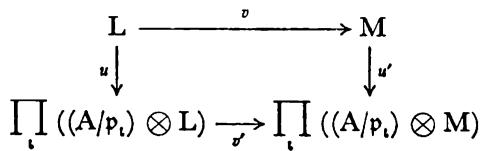
\includegraphics[keepaspectratio]{images/part001_964082be.jpg}}

where \(u\) (resp. \(u'\) ) is the mapping \(x \mapsto (\phi_{\iota}(x))\) (resp. \(y \mapsto (\psi_{\iota}(y)))\) ,

\[
\phi_ {i} \colon \mathbf {L} \rightarrow (\mathbf {A} / \mathfrak {p} _ {i}) \otimes \mathbf {L}
\]

(resp. \(\psi_{t}\colon\mathbf{M}\to(\mathbf{A}/p_{t})\otimes\mathbf{M}\) ) being the canonical mapping, and \(v'\) is the product of the \(1_{\mathbf{A}/p_{t}}\otimes v\) . Then \((\mathbf{A}/p)/(m/p_{t})\otimes_{\mathbf{A}/p_{t}}((\mathbf{A}/p_{t})\otimes_{\mathbf{A}}\mathbf{M})=(\mathbf{A}/m)\otimes_{\mathbf{A}}\mathbf{M}\) and, as \(A/p_{t}\) is a local integral domain, it follows from the first part of the argument that each of the \(1_{\mathbf{A}/p_{t}}\otimes v\) is an isomorphism; then so is \(v'\) . On the other hand, as A is reduced, \(\bigcap_{i} p_{i} = (0)\) ( \(\S 2\) , no. 6, Proposition 13), whence \(\bigcap_{i} (p_{i} L) = 0\) since L is free (Algebra, Chapter II, \(\S 3\) , no. 7, Remark); as \(p_{i} L\) is the kernel of \(\phi_{i}\) , this shows that \(u\) is injective. It follows that \(v' \circ u = u' \circ v\) is injective, hence \(v\) is injective and, as \(v\) is surjective by definition, this shows that M is free.

\subsection{Passage from the local to the global}

PROPOSITION 8. Let A be a ring, m a maximal ideal of A and M an A-module. If there exists an ideal a of A such that m is the only maximal ideal of A containing a and aM = 0, then the canonical homomorphism \(M \rightarrow M_{m}\) is bijective.

A/a is then a local ring with maximal ideal m/a; M can be considered as an (A/a)-module; for all \(s \in A - m\) the canonical image of s in A/a is invertible, hence the homothety \(x \mapsto sx\) of M is bijective from the definition of \(M_{m}\) as the solution of a universal problem (§ 2, no. 2); whence the proposition.

In particular, if there exists \(k \geqslant 0\) such that \(\mathfrak{m}^k\mathbf{M} = 0\) , the homomorphism \(\mathbf{M} \to \mathbf{M}_m\) is bijective (§ 1, no. 1, Corollary to Proposition 1).

PROPOSITION 9. Let A be a ring, m a maximal ideal of A, M an A-module and k an integer \(\geqslant0\) . The canonical homomorphism \(M\to M_{m}/m^{k}M_{m}\) is surjective, has kernel \(m^{k}M\) and defines an isomorphism of \(M/m^{k}M\) onto \(M_{m}/m^{k}M_{m}\) .

Since the case \(k=0\) is trivial, suppose that \(k\geqslant1\) . It follows from Proposition 8 that the canonical homomorphism \(\mathbf{M}/\mathfrak{m}^{k}\mathbf{M}\to(\mathbf{M}/\mathfrak{m}^{k}\mathbf{M})_{\mathfrak{m}}\) is bijective. On the other hand \((\mathbf{M}/\mathfrak{m}^{k}\mathbf{M})_{\mathfrak{m}}\) is canonically identified with \(\mathbf{M}_{\mathfrak{m}}/(\mathfrak{m}^{k}\mathbf{M})_{\mathfrak{m}}\) (§2, no. 4, Theorem 1) and hence \((\mathfrak{m}^{k}\mathbf{M})_{\mathfrak{m}}=\mathfrak{m}^{k}\mathbf{M}_{\mathfrak{m}}\) (§2, no. 7, Corollary to Proposition 18), whence there is an isomorphism of \(\mathbf{M}/\mathfrak{m}^{k}\mathbf{M}\) onto \(\mathbf{M}_{\mathfrak{m}}/\mathfrak{m}^{k}\mathbf{M}_{\mathfrak{m}}\) which maps the class of an element \(x\in\mathbf{M}\) to the class of \(x/1\) .

COROLLARY. Let A be a ring, \(m_{1}, m_{2}, \ldots, m_{n}\) distinct maximal ideals of A, M an A-module and \(k_{1}, k_{2}, \ldots, k_{n}\) integers \(\geqslant 0\) . The canonical homomorphism from M to \(\prod_{i=1}^{n} \mathbf{M}_{\mathfrak{m}_{i}}/\mathfrak{m}_{i}^{k_{i}} \mathbf{M}_{\mathfrak{m}_{i}}\) is surjective and its kernel is \(\left(\bigcap_{i=1}^{n} \mathfrak{m}_{i}^{k_{i}}\right) \mathbf{M}\) .

This follows easily from Proposition 9 and §1, no. 2, Proposition 6, the \(\mathfrak{m}_{i}^{k_{i}}\) being relatively prime in pairs (§1, no. 2, Proposition 3).

In the rest of this no. A will denote a ring and \(\Omega(A)\) (or \(\Omega\) ) the set of maximal ideals of \(A\) .

PROPOSITION 10. The A-module \(\bigoplus_{m\in\Omega}A_m\) , the direct sum of the \(A_m\) , where \(m\in\Omega\) , is faithfully flat.

Each of the \(A_{m}\) is a flat A-module ( \(\S\) 2, no. 4, Theorem 1), hence \(E = \bigoplus_{m \in \Omega} A_{m}\) is flat (Chapter I, \(\S\) 2, no. 3, Proposition 2). Moreover, for every maximal ideal m of A, \(mA_{m}\) is the unique maximal ideal of \(A_{m}\) , hence \(mA_{m} \neq A_{m}\) , whence it follows that \(mE \neq E\) and consequently E is faithfully flat (Chapter I, \(\S\) 3, no. 1, Proposition 1 (d)).

THEOREM 1. Let M, N be two A-modules, \(u: \mathbf{M} \to \mathbf{N}\) an A-homomorphism and, for all \(m \in \Omega\) , let \(u_m: \mathbf{M}_m \to \mathbf{N}_m\) be the corresponding \(\mathbf{A}_m\) -homomorphism (§ 2, no. 2, Remark 5). For \(u\) to be injective (resp. surjective, bijective, zero), it is necessary and sufficient that, for all \(m \in \Omega\) , \(u_m\) be injective (resp. surjective, bijective, zero).

To say that, for all \(m \in \Omega\) , \(u_m\) is injective (resp. surjective, bijective, zero) is equivalent to saying that the homomorphism \(\bigoplus_{m} u_m: \bigoplus_{m} M_m \to \bigoplus_{m} N_m\) has the same property. But \(\bigoplus_{m} M_m = M \otimes_A E\) , \(\bigoplus_{m} N_m = N \otimes_A E\) and \(\bigoplus_{m} u_m = u \otimes 1\) , where \(E = \bigoplus_{m} A_m\) ; as \(E\) is faithfully flat (Proposition 10), the theorem follows from Chapter I, § 3, no. 1, Proposition 1 (c) and Proposition 2.

COROLLARY 1. Let M be an A-module, N a submodule of M and x an element of M. For \(x \in N\) , it is necessary and sufficient that, for all \(m \in \Omega\) , the canonical image of x in \(M_{m}\) belong to \(N_{m}\) .

Let \(\bar{x}\) be the class of \(x\) in M/N; to say that \(x \in N\) means that the A-linear mapping \(u: \alpha \mapsto \alpha \bar{x}\) from A to M/N is zero. Now, \((\mathrm{M} / \mathrm{N})_{\mathfrak{m}}\) is identified with \(\mathrm{M}_{\mathfrak{m}} / \mathrm{N}_{\mathfrak{m}}\) (§ 2, no. 4, Theorem 1) and \(u_{\mathfrak{m}}: \mathrm{A}_{\mathfrak{m}} \to \mathrm{M}_{\mathfrak{m}} / \mathrm{N}_{\mathfrak{m}}\) with the mapping \(\lambda \mapsto \lambda \bar{x}_{\mathfrak{m}}\) , where \(\bar{x}_{\mathfrak{m}}\) is the class mod. \(\mathrm{N}_{\mathfrak{m}}\) of the canonical image of \(x\) in \(\mathrm{M}_{\mathfrak{m}}\) . As the relation \(u = 0\) is equivalent to \(u_{\mathfrak{m}} = 0\) for all m by Theorem 1, this proves the corollary.

COROLLARY 2. Let \(\mathbf{M}\) be an A-module and, for all \(\mathfrak{m} \in \Omega\) , let \(f_{\mathfrak{m}}\) be the canonical mapping \(\mathbf{M} \to \mathbf{M}_{\mathfrak{m}}\) . The homomorphism \(x \mapsto (f_{\mathfrak{m}}(x))\) of \(\mathbf{M}\) to \(\prod_{\mathfrak{m} \in \Omega} \mathbf{M}_{\mathfrak{m}}\) is injective.

Applying Corollary 1 in the case N = 0, it is seen that the relation x = 0 is equivalent to \(f_{m}(x) = 0\) for all \(m \in \Omega\) .

COROLLARY 3. (i) Let \(\mathfrak{b}\) be an ideal of \(\mathbf{A}\) and a an element of \(\mathbf{A}\) . For \(a \in \mathfrak{b}\) , it is necessary and sufficient that, for all \(\mathfrak{m} \in \Omega\) , the canonical image of \(a\) in \(\mathbf{A}_{\mathfrak{m}}\) belong to \(\mathfrak{b}\mathbf{A}_{\mathfrak{m}}\) .

\begin{enumerate}
\def\labelenumi{(\roman{enumi})}
\setcounter{enumi}{1}
\tightlist
\item
  In particular, let \(b\) and \(c\) be two elements of \(A\) . For \(c\) to be a multiple of \(b\) , it is necessary and sufficient that, for all \(m \in \Omega\) , the canonical image of \(c\) in \(A_m\) be a multiple of that of \(b\) .
\end{enumerate}

As \(\mathfrak{bA}_{m} = \mathfrak{b}_{m}\) (§ 2, no. 7, Corollary to Proposition 18), (i) is a special case of Corollary 1; (ii) follows from (i) applied to the ideal Ab.

COROLLARY 4. Let A be an integral domain, K its field of fractions and M a torsion-free A-module such that M is canonically identified with a sub-A-module of \(\mathbf{K} \otimes_{\mathbf{A}} \mathbf{M}\) . Then, for all \(\mathfrak{m} \in \Omega\) , \(\mathbf{M}_{\mathfrak{m}}\) is canonically identified with a sub-A-module of \(\mathbf{K} \otimes_{\mathbf{A}} \mathbf{M}\) and \(\mathbf{M} = \bigcap_{\mathfrak{m} \in \Omega} \mathbf{M}_{\mathfrak{m}}\) .

As M is identified with a submodule of \(K \otimes_{A} M\) , \(M_{m}\) is identified with a sub- \(A_{m}\) -module of \((\mathbf{K} \otimes_{\mathbf{A}} \mathbf{M})_{\mathfrak{m}} = \mathbf{K}_{\mathfrak{m}} \otimes_{\mathbf{A}} \mathbf{M}\) (§2, no. 4, Theorem 1); as \(K_{m} = K\) , we see straightway that \(M_{m}\) is torsion-free; moreover, the commutativity of the diagram

\[
\begin{array}{c} \mathbf {M} \longrightarrow \mathbf {K} \otimes_ {\mathbf {A}} \mathbf {M} \\ \Big \downarrow \qquad \qquad \qquad \qquad \qquad \qquad \qquad \qquad \Big \downarrow \\ \mathbf {M} _ {\mathfrak {m}} \longrightarrow (\mathbf {K} \otimes_ {\mathbf {A}} \mathbf {M}) _ {\mathfrak {m}} \end{array}
\]

proves that the canonical mapping \(M \rightarrow M_{m}\) is injective. The corollary then follows from Corollary 1 applied to the A-module \(K \otimes_{A} M\) and its submodule M.

In particular, for every integral domain A,

\[
\mathbf {A} = \bigcap_ {\mathfrak {m} \in \Omega} \mathbf {A} _ {\mathfrak {m}}.\tag{2}
\]

COROLLARY 5. Let A be a ring. Every system of generators of the A-module \(\mathbf{A}^n\) with \(n\) elements is a basis of \(\mathbf{A}^n\) .

Let \((e_i)_{1\leqslant i\leqslant n}\) be the canonical basis of \(\mathbf{A}^n\) , \((x_i)_{1\leqslant i\leqslant n}\) a system of generators of \(\mathbf{A}^n\) with \(n\) elements and \(u\colon \mathbf{A}^n\to \mathbf{A}^n\) the A-linear mapping such that \(u(e_i) = x_i\) for \(1\leqslant i\leqslant n\) . By hypothesis \(u\) is surjective and it is necessary to show that \(u\) is injective. By virtue of Theorem 1 this can immediately be reduced to the case where \(\mathbf{A}\) is a local ring; if \(\mathfrak{m}\) is the maximal ideal of \(\mathbf{A}\) , the elements \(1\otimes x_i\) ( \(1\leqslant i\leqslant n\) ) in \((\mathrm{A / m})^n\) then form a system of generators of the free \((\mathrm{A / m})\) -module \((\mathrm{A / m})^n\) ; as \(\mathrm{A / m}\) is a field, this system is a basis of \((\mathrm{A / m})^n\) ; as \(\mathbf{A}^n\) is a free A-module, we deduce from Proposition 5 that \((x_i)\) is a basis of \(\mathbf{A}^n\) .

PROPOSITION 11. Let M be an A-module, N a finitely generated A-module and \(u: \mathbf{M} \to \mathbf{N}\) a homomorphism. For \(u\) to be surjective, it is necessary and sufficient that, for all \(\mathfrak{m} \in \Omega\) , the homomorphism \(\mathbf{M} / \mathfrak{m}\mathbf{M} \to \mathbf{N} / \mathfrak{m}\mathbf{N}\) derived from \(u\) by taking quotients be surjective.

It follows from Theorem 1 that, for \(u\) to be surjective, it is necessary and sufficient that \(u_{\mathfrak{m}}: \mathrm{M}_{\mathfrak{m}} \to \mathrm{N}_{\mathfrak{m}}\) be surjective for all \(\mathfrak{m} \in \Omega\) . As \(\mathrm{A}_{\mathfrak{m}}\) is a local ring and \(\mathrm{N}_{\mathfrak{m}}\) is a finitely generated \(\mathrm{A}_{\mathfrak{m}}\) -module, this amounts to saying that the homomorphism \(u_{\mathfrak{m}}': \mathrm{M}_{\mathfrak{m}} / \mathrm{mM}_{\mathfrak{m}} \to \mathrm{N}_{\mathfrak{m}} / \mathrm{mN}_{\mathfrak{m}}\) , obtained by taking quotients, is surjective (no. 2, Corollary 1 to Proposition 4); but \(\mathrm{M}_{\mathfrak{m}} / \mathrm{mM}_{\mathfrak{m}}\) (resp. \(\mathrm{N}_{\mathfrak{m}} / \mathrm{mN}_{\mathfrak{m}}\) ) is identified with \(\mathrm{M} / \mathrm{mM}\) (resp. \(\mathrm{N} / \mathrm{mN}\) ) (Proposition 9), whence the proposition.

PROPOSITION 12. Let E, F, G be three A-modules and \(v: \mathbf{G} \to \mathbf{F}\) , \(u: \mathbf{E} \to \mathbf{F}\) homomorphisms. Suppose that E is finitely presented. For there to exist a homomorphism \(w: \mathbf{E} \to \mathbf{G}\) such that \(u\) factors into \(\mathbf{E} \xrightarrow{w} \mathbf{G} \xrightarrow{v} \mathbf{F}\) , it is necessary and sufficient that, for all \(m \in \Omega\) , there exist a homomorphism \(w^m: \mathbf{E}_m \to \mathbf{G}_m\) such that \(u_m: \mathbf{E}_m \to \mathbf{F}_m\) factors into \(\mathbf{E}_m \xrightarrow{w^m} \mathbf{G}_m \xrightarrow{v_m} \mathbf{F}_m\) .

The existence of w satisfying the above statement is equivalent to the following property: u belongs to the image P of the mapping

\[
r = \operatorname{Hom} (1 _ {\mathbf {E}}, v): \operatorname{Hom} _ {\mathbf {A}} (\mathbf {E}, \mathbf {G}) \rightarrow \operatorname{Hom} _ {\mathbf {A}} (\mathbf {E}, \mathbf {F}).
\]

Now, \((\mathrm{Hom}_{\mathbf{A}}(\mathrm{E},\mathbf{F}))_{\mathfrak{m}}\) (resp. \((\mathrm{Hom}_{\mathbf{A}}(\mathrm{E},\mathbf{G}))_{\mathfrak{m}}\) ) is canonically identified with \(\mathrm{Hom}_{\mathbf{A}_{\mathfrak{m}}}(\mathrm{E}_{\mathfrak{m}},\mathrm{F}_{\mathfrak{m}})\) (resp. \(\mathrm{Hom}_{\mathbf{A}_{\mathfrak{m}}}(\mathrm{E}_{\mathfrak{m}},\mathrm{G}_{\mathfrak{m}})\) ) (§ 2, no. 7, Proposition 19 (i)), the canonical image of u in \((\mathrm{Hom}_{\mathbf{A}}(\mathrm{E},\mathbf{F}))_{\mathfrak{m}}\) is identified with \(u_{m}\) , \(r_{m}\) is identified with \(\mathrm{Hom}_{\mathbf{A}_{\mathfrak{m}}}(1_{\mathbf{E}_{\mathfrak{m}}},v_{\mathfrak{m}})\) and \(P_{m}\) with the image of \(r_{m}\) . The proposition then follows from Corollary 1 to Theorem 1 applied to \(\mathrm{Hom}_{\mathbf{A}}(\mathrm{E},\mathbf{F})\) and its submodule P.

COROLLARY 1. Let M be an A-module and N a submodule of M such that M/N is finitely presented. For N to be a direct factor of M, it is necessary and sufficient that, for all \(m \in \Omega\) , \(N_{m}\) be a direct factor of \(M_{m}\) .

To say that N is a direct factor of M means that the identity homomorphism on M/N factors into \(M/N \xrightarrow{w} M \xrightarrow{\phi} M/N\) where \(\phi\) is the canonical homomorphism and w a homomorphism (Algebra, Chapter II, § 1, no. 9, Proposition 14); as \((\mathrm{M}/\mathrm{N})_{\mathrm{m}} = \mathrm{M}_{\mathrm{m}}/\mathrm{N}_{\mathrm{m}}\) and \(\phi_{m}\) is the canonical homomorphism \(M_{m} \to M_{m}/N_{m}\) , the corollary follows easily from Proposition 12.

COROLLARY 2. Let M be a finitely generated free A-module and N a submodule of M which is a finitely generated free A-module. For N to be a direct factor of M, it is necessary and sufficient that, for all m ∈ Ω, mN = N ∩ (mM).

By definition M/N is finitely presented; on the other hand, \(N_{m}\) and \(M_{m}\) are finitely generated free \(A_{m}\) -modules. For \(N_{m}\) to be a direct factor of \(M_{m}\) , it is necessary and sufficient that the canonical mapping \(N_{m}/mN_{m} \rightarrow M_{m}/mM_{m}\) be injective (no. 2, Proposition 6); this is the same as saying that the canonical mapping \(N/mN \rightarrow M/mM\) must be injective (Proposition 9), and as its kernel is \((N \cap mM)/mN\) , this proves the corollary.

Proposition 12 (resp. its Corollary 1) will be applied in particular when A is Noetherian and E (resp. M/N) a finitely generated A-module (Chapter I, § 2, no. 8, Lemma 8).

\subsection{Localization of flatness}

PROPOSITION 13. Let S be a multiplicative subset of a ring A and M an A-module. If M is flat (resp. faithfully flat), \(S^{-1}M\) is a flat (resp. faithfully flat) \(S^{-1}A\) -module and a flat A-module.

As \(S^{-1}M = M \otimes_{A} S^{-1}A\) , the first assertion follows from Chapter I, §2, no. 7, Corollary 2 to Proposition 8 (resp. Chapter I, §3, no. 3, Proposition 5); moreover, \(S^{-1}A\) is a flat A-module (§2, no. 4, Theorem 1); hence if M is a flat A-module, so is \(S^{-1}M\) by virtue of Chapter I, §2, no. 7, Corollary 3 to Proposition 8.

Remark. If N is an \(S^{-1}A\) -module, \(S^{-1}N\) is identified with N and this is consequently equivalent to saying that N is a flat \(S^{-1}A\) -module or a flat A-module.

PROPOSITION 14. Let A be a ring, B a commutative A-algebra and T a multiplicative subset of B. If N is a B-module which is flat as an A-module, \(T^{-1}N\) is a flat A-module.

\(T^{-1}N = T^{-1}B \otimes_{B} N\) ; the proposition then follows from Chapter I, § 2, no. 7, Proposition 8, applied with A replaced by B, B by A, E by \(T^{-1}B\) and F by N.

PROPOSITION 15. Let A, B be two rings, \(\phi: A \to B\) a homomorphism and N a B-module. The following properties are equivalent:

\begin{enumerate}
\def\labelenumi{(\alph{enumi})}
\item
  N is a flat A-module.
\item
  For every maximal ideal \(\mathfrak{n}\) of \(\mathbf{B}\) , \(\mathbf{N}_{\mathfrak{n}}\) is a flat A-module.
\item
  For every maximal ideal \(\mathfrak{n}\) of \(\mathbf{B}\) , if we write \(\mathfrak{m} = \bar{\phi}^{-1}(\mathfrak{n})\) , \(\mathbf{N}_{\mathfrak{n}}\) is a flat \(\mathbf{A}_{\mathfrak{m}}\) -module.
\end{enumerate}

For all \(a \notin m\) , the homothety of \(N_{n}\) induced by a is bijective, hence \(N_{n}\) is canonically identified with \((\mathrm{N}_{\mathrm{n}})_{\mathrm{m}}\) and the equivalence of (b) and (c) follows from the

Remark following Proposition 13; the fact that (a) implies (b) is a special case of Proposition 14. It remains to prove that (b) implies (a), that is, that, if (b) holds, for every injective A-module homomorphism \(u: \mathbf{M} \to \mathbf{M}'\) , the homomorphism \(v = 1 \otimes u: \mathbf{N} \otimes_{\mathbf{A}} \mathbf{M} \to \mathbf{N} \otimes_{\mathbf{A}} \mathbf{M}'\) is injective. Now, \(v\) is also a B-module homomorphism and, for it to be injective, it is necessary and sufficient that \(v_n: (\mathbf{N} \otimes_{\mathbf{A}} \mathbf{M})_n \to (\mathbf{N} \otimes_{\mathbf{A}} \mathbf{M}')_n\) be so for every maximal ideal \(n\) of \(B\) (no. 3, Theorem 1). As

\[
(\mathbf {N} \otimes_ {\mathbf {A}} \mathbf {M}) _ {n} = \mathbf {B} _ {n} \otimes_ {\mathbf {B}} (\mathbf {N} \otimes_ {\mathbf {A}} \mathbf {M}) = \mathbf {N} _ {n} \otimes_ {\mathbf {A}} \mathbf {M},
\]

\(v_{n}\) is just the homomorphism \(1 \otimes u: N_{n} \otimes_{A} M \to N_{n} \otimes_{A} M'\) , which is injective since \(N_{n}\) is a flat A-module by hypothesis.

COROLLARY. For an A-module M to be flat (resp. faithfully flat), it is necessary and sufficient that, for every maximal ideal m of A, \(M_{m}\) be a flat (resp. faithfully flat) \(A_{m}\) -module.

The necessity of the conditions follows from Proposition 13. Conversely, if \(M_{m}\) is a flat \(A_{m}\) -module for every maximal ideal m of A, M is a flat A-module by virtue of Proposition 15 applied to the case where \(\phi\) is the identity. Finally, if \(M_{m}\) is a faithfully flat \(A_{m}\) -module for all m, then \(mM_{m} = mA_{m}M_{m} \neq M_{m}\) , hence \(mM \neq M\) for all m (no. 3, Proposition 9), which proves that M is a faithfully flat A-module (Chapter I, § 3, no. 1, Proposition 1 (d)).

\subsection{Semi-local rings}

PROPOSITION 16. Let A be a ring. The following properties are equivalent:

\begin{enumerate}
\def\labelenumi{(\alph{enumi})}
\item
  the set of maximal ideals of \(\mathbf{A}\) is finite;
\item
  the quotient of A by its Jacobson radical is the direct composition of a finite number of fields.
\end{enumerate}

Suppose that the quotient of A by its Jacobson radical \(\Re\) is a direct composition of a finite number of fields. Then A/ \(\Re\) possesses only a finite number of ideals and \(a\ fortiori\) only a finite number of maximal ideals. As every maximal ideal contains \(\Re\) (Algebra, Chapter VIII, § 6, no. 2, Definition 2), the maximal ideals of A are the inverse images of the maximal ideals of A/ \(\Re\) under the canonical homomorphism A \(\rightarrow\) A/ \(\Re\) ; hence they are finite in number.

Conversely, suppose that A has only a finite number of distinct maximal ideals \(m_{1}, \ldots, m_{n}\) . The \(A/m_{i}\) are fields and it follows from § 1, no. 2, Proposition 5 that the canonical mapping \(A \to \prod_{i=1}^{n} A/m_{i}\) is surjective; as its kernel \(\bigcap_{i=1}^{n} m_{i}\) is the Jacobson radical R (Algebra, Chapter VIII, § 6, no. 2, Definition 2), A/R is isomorphic to \(\prod_{i=1}^{n} A/m_{i}\) .

DEFINITION 4. A ring is called semi-local if it satisfies the equivalent conditions (a), (b) of Proposition 16.

Examples. Every local ring is semi-local. Every quotient of a semi-local ring is semi-local. Every finite product of semi-local rings is semi-local.

* If A is a Noetherian semi-local ring and B is an A-algebra which is a finitely generated A-module, then B is semi-local (Chapter IV, § 2, no. 5, Corollary 3 to Proposition 9). *

Another example, generalizing the construction of the local rings \(A_{p}\) , is provided by the following proposition:

PROPOSITION 17. Let A be a ring and \(p_1, \ldots, p_n\) prime ideals of A. We write \(S = \bigcap_{i=1}^{n} (A - p_i) = A - \bigcup_{i=1}^{n} p_i\) .

\begin{enumerate}
\def\labelenumi{(\alph{enumi})}
\item
  The ring \(\mathbf{S}^{-1}\mathbf{A}\) is semi-local; if \(\mathfrak{q}_1, \ldots, \mathfrak{q}_r\) are the distinct maximal elements (with respect to inclusion) of the set of \(\mathfrak{p}_i\) , the maximal ideals of \(\mathbf{S}^{-1}\mathbf{A}\) are the \(\mathbf{S}^{-1}\mathfrak{q}_j\) ( \(1 \leqslant j \leqslant r\) ) and these ideals are distinct.
\item
  The ring \(\mathbf{A}_{\mathfrak{p}_i}\) is canonically isomorphic to \((\mathbf{S}^{-1}\mathbf{A})_{\mathbf{S}^{-1}\mathfrak{p}_i}\) for \(1 \leqslant i \leqslant n\) .
\item
  If \(\mathbf{A}\) is an integral domain, then \(\mathbf{S}^{-1}\mathbf{A} = \bigcap_{i=1}^{n}\mathbf{A}_{p_i}\) in the field of fractions of \(\mathbf{A}\) .
\end{enumerate}

(a) The ideals of A not meeting S are the ideals contained in the union of the \(p_{i}\) and hence in at least one of the \(p_{i}\) (§ 1, no. 1, Proposition 2); the \(q_{j}\) are therefore the maximal elements of the set of ideals not meeting S; consequently, the \(S^{-1}q_{j}\) are the maximal ideals of \(S^{-1}A\) by § 2, no. 5, Proposition 11 (ii).

(b) is a special case of § 2, no. 5, Proposition 11 (iii).

(c) Suppose that A is an integral domain. If \(p_{i} \subset p_{k}\) , then \(A_{p_{i}} \supset A_{p_{k}}\) ; to prove (c), we may therefore suppose that no two \(p_{i}\) are comparable. Then it follows from (a) and no. 3, Corollary 4 to Theorem 1 that \(S^{-1}A = \bigcap_{i=1}^{n} (S^{-1}A)_{S^{-1}p_{i}}\) ; whence (c) by virtue of (b).

If A is an integral domain, so is \(S^{-1}A\) and Proposition 17 then provides an example of a semi-local ring which is not a direct composition of local rings (cf.~Chapter III, § 2, no. 13).

COROLLARY. Let A be an integral domain and \(p_{1}, \ldots, p_{n}\) prime ideals of A, no two of which are comparable with respect to inclusion. If \(A = \bigcap_{i=1}^{n} A_{p_{i}}\) in the field of fractions of A, the maximal ideals of A are \(p_{1}, \ldots, p_{n}\) .

Setting \(S = \bigcap_{i=1}^{n} (A - p_i), S^{-1} A = A\) by Proposition 17 (c); hence the elements of \(S\) are invertible in \(A\) and \(S^{-1} p_i = p_i\) for all \(i\) . Our assertion then follows by virtue of Proposition 17 (a).

\section{SPECTRA OF RINGS AND SUPPORTS OF MODULES}

\subsection{Irreducible spaces}

DEFINITION 1. A topological space X is called irreducible if every finite intersection of non-empty open sets of X is non-empty.

By considering the empty family of open sets of X it is seen that an irreducible space is non-empty; for a topological space X to be irreducible, it is necessary and sufficient that it be non-empty and that the intersection of two non-empty open sets of X be always non-empty (or, what amounts to the same thing, that the union of two closed sets distinct from X be always distinct from X).

PROPOSITION 1. Let X be a non-empty topological space. The following conditions are equivalent:

\begin{enumerate}
\def\labelenumi{(\alph{enumi})}
\item
  \(\mathbf{X}\) is irreducible;
\item
  every non-empty open set of \(\mathbf{X}\) is dense in \(\mathbf{X}\) ;
\item
  every open set of \(\mathbf{X}\) is connected.
\end{enumerate}

By definition, a set which is dense in X is a set which meets every non-empty open set, hence (a) and (b) are equivalent. It is immediate that (c) implies (a), for if \(U_{1}\) and \(U_{2}\) are disjoint non-empty open sets, \(U_{1} \cup U_{2}\) is a disconnected open set. Finally let us show that (a) implies (c): if U is a disconnected open set, it is the union of two disjoint non-empty sets \(U'\) , \(U''\) which are open in U and hence also open in X, which implies that X is not irreducible.

A Hausdorff space is irreducible only if it consists of a single point.

A subset E of a topological space X is called an irreducible set if the subspace E of X is irreducible. For this to be so, it is necessary and sufficient that, for every pair of sets U, V which are open in X and meet E, \(U \cap V\) also meet E, or (what amounts to the same thing) that, for every pair of sets F, G which are closed in X and satisfy \(E \subset F \cup G\) , \(E \subset F\) or \(E \subset G\) . By induction on n, we deduce that, if \((\mathbf{F}_{i})_{1 \leq i \leq n}\) is a finite family of closed sets of X such that \(E \subset \bigcup_{i=1}^{n} F_{i}\) , there exists an index i such that \(E \subset F_{i}\) .

PROPOSITION 2. In a topological space X, for a set E to be irreducible, it is necessary and sufficient that its closure \(\overline{E}\) be so.

For an open set of X to meet E, it is necessary and sufficient that it meet \(\overline{E}\) ; then the proposition follows from the above remarks.

PROPOSITION 3. (i) If X is an irreducible space, every non-empty open subset of X is irreducible.

\begin{enumerate}
\def\labelenumi{(\roman{enumi})}
\setcounter{enumi}{1}
\item
  Let \((\mathbf{U}_{\alpha})_{\alpha \in \mathbf{A}}\) be a non-empty covering of a topological space \(\mathbf{X}\) consisting of open sets such that \(\mathbf{U}_{\alpha} \cap \mathbf{U}_{\beta} \neq \varnothing\) for every pair of indices \((\alpha, \beta)\) . If the sets \(\mathbf{U}_{\alpha}\) are irreducible, the space \(\mathbf{X}\) is irreducible.
\end{enumerate}

(i) If \(\mathbf{X}\) is irreducible, \(\mathbf{U} \subset \mathbf{X}\) non-empty and open in \(\mathbf{X}\) and \(\mathbf{V} \subset \mathbf{U}\) non-empty and open in \(\mathbf{U}\) , \(\mathbf{V}\) is also open in \(\mathbf{X}\) , therefore dense in \(\mathbf{X}\) and a fortiori dense in \(\mathbf{U}\) . Then \(\mathbf{U}\) is irreducible (Proposition 1).

(ii) Let us show that, for every non-empty open set V in X, \(V \cap U_{\alpha} \neq \varnothing\) for all \(\alpha \in A\) : it follows that \(V \cap U_{\alpha}\) is dense in \(U_{\alpha}\) by hypothesis, hence that V is dense in X and this proves that X is irreducible (Proposition 1). Now there exists at least one index \(\gamma\) such that \(V \cap U_{\gamma} \neq \varnothing\) ; as \(U_{\alpha} \cap U_{\gamma} \neq \varnothing\) for all \(\alpha\) and \(V \cap U_{\gamma}\) is dense in \(U_{\gamma}\) , \(U_{\alpha} \cap U_{\gamma} \cap V \neq \varnothing\) and a fortiori \(U_{\alpha} \cap V \neq \varnothing\) , which completes the proof of (ii).

PROPOSITION 4. Let X and Y be two topological spaces and f a continuous mapping from X to Y. For every irreducible subset E of X, \(f(E)\) is an irreducible subset of Y.

If U, V are two open sets of Y which meet \(f(\mathrm{E})\) , \(\overline{f}^{-1}(\mathrm{U})\) and \(\overline{f}^{-1}(\mathrm{V})\) are open sets of X which meet E. Consequently, \(\overline{f}^{-1}(\mathrm{U}) \cap \overline{f}^{-1}(\mathrm{V}) = \overline{f}^{-1}(\mathrm{U} \cap \mathrm{V})\) meets E, which implies that \(U \cap V\) meets \(f(\mathrm{E})\) and proves the proposition.

DEFINITION 2. Every maximal irreducible subset of a topological space X is called an irreducible component of X.

It follows from Proposition 2 that every irreducible component of \(\mathbf{X}\) is closed in \(\mathbf{X}\) .

PROPOSITION 5. Let X be a topological space. Every irreducible subset of X is contained in an irreducible component of X and X is the union of its irreducible components.

To prove the first assertion, it is sufficient, by virtue of Zorn's Lemma, to prove that the set \(\Im\) of irreducible subsets of \(X\) is inductive. Let \(\mathfrak{G}\) be a subset of \(\Im\) totally ordered by inclusion; we show that the union \(E\) of the sets \(F \in \mathfrak{G}\) is irreducible. Let \(U\) , \(V\) be two open sets of \(X\) which meet \(E\) ; as \(\mathfrak{G}\) is totally ordered, there exists a set \(F \in \mathfrak{G}\) meeting U and V; as F is irreducible, \(U \cap V\) meets F and hence also E, which proves that E is irreducible and hence that \(\mathfrak{G}\) is inductive. The second assertion follows from the first, for every subset of X consisting of a single point is irreducible.

COROLLARY. Every connected component of a topological space X is a union of irreducible components of X.

Every irreducible subspace of X is connected by Proposition 1 and hence is contained in a connected component of X.

Note that two distinct irreducible components of X may have points in common (Exercise 11).

PROPOSITION 6. Let X be a topological space and \((\mathrm{P}_{i})_{1\leq i\leq n}\) a finite covering of X consisting of irreducible closed sets. Then the irreducible components of X are the maximal elements (with respect to inclusion) of the set of \(P_{i}\) .

We may restrict ourselves to the case where no two \(P_{i}\) are comparable. If E is an irreducible subset of X, then \(E \subset \bigcup_{i=1}^{n} P_{i}\) and hence E is contained in one of the closed sets \(P_{i}\) ; this proves that the \(P_{i}\) are the only maximal irreducible subsets of X.

COROLLARY. Let X be a topological space and E a subspace with only a finite number of distinct irreducible components \(Q_{i}\) ( \(1 \leqslant i \leqslant n\) ); then the irreducible components of the closure \(\overline{E}\) in X are the closures \(\overline{Q}_{i}\) of the \(Q_{i}\) ( \(1 \leqslant i \leqslant n\) ) and \(\overline{Q}_{i} \neq \overline{Q}_{j}\) for \(i \neq j\) .

\(\overline{\mathbf{E}}\) is the union of the \(\overline{\mathbf{Q}}_i\) , which are irreducible (Proposition 2); as \(\mathbf{Q}_i\) is closed in \(\mathbf{E}\) , \(\overline{\mathbf{Q}}_i \cap \mathbf{E} = \mathbf{Q}_i\) ; as \(\mathbf{Q}_i \not\subset \mathbf{Q}_j\) for \(i \neq j\) , \(\overline{\mathbf{Q}}_i \not\subset \overline{\mathbf{Q}}_j\) , whence the corollary by virtue of Proposition 6.

Remark. Suppose that X has only a finite number of distinct irreducible components \(X_{i}\) ( \(1 \leqslant i \leqslant n\) ); then \(U_{i} = \complement\left(\bigcup_{j \neq i} X_{j}\right)\) is open in X and dense in \(X_{i}\) since \(X_{i} \not\subset \bigcup_{j \neq i} X_{j}\) ; the \(U_{i}\) ( \(1 \leqslant i \leqslant n\) ) are therefore non-empty open sets of X which are irreducible (Proposition 2), pairwise disjoint and with their union dense in X.

PROPOSITION 7. Let U be an open subset of a topological space X. The mapping \(V \mapsto \overline{V}\) (closure in X) is a bijection of the set of irreducible subsets of U which are closed in U onto the set of irreducible subsets of X which are closed in X and meet U; the inverse bijection is \(Z \mapsto Z \cap U\). In particular, this bijection maps the set of irreducible components of U onto the set of irreducible components of X which meet U.

If V is closed in U and irreducible, \(\overline{V}\) is irreducible (Proposition 2) and \(V = \overline{V} \cap U\) . Conversely, if Z is irreducible and closed in X and meets U, \(Z \cap U\) is a non-empty open subset of Z, hence irreducible (Proposition 3) and dense in Z and, as Z is closed, \(Z = \overline{Z \cap U}\) . This proves the proposition.

\subsection{Noetherian topological spaces}

DEFINITION 3. A topological space X is called Noetherian if every non-empty set of closed subsets of X, ordered by inclusion, has a minimal element.

It amounts to the same to say that every non-empty set of open subsets of X, ordered by inclusion, has a maximal element, or that every decreasing (resp. increasing) sequence of closed (resp. open) sets is stationary (Set Theory, Chapter III, § 6, no. 5, Proposition 6).

PROPOSITION 8. (i) Every subspace of a Noetherian space is Noetherian.

\begin{enumerate}
\def\labelenumi{(\roman{enumi})}
\setcounter{enumi}{1}
\item
  Let \((\mathbf{A}_i)_{i\in I}\) be a finite covering of a topological space \(\mathbf{X}\) . If the subspaces \(\mathbf{A}_i\) of \(\mathbf{X}\) are Noetherian, \(\mathbf{X}\) is Noetherian.

\end{enumerate}

(i) Let X be a Noetherian space, A a subspace of X and \((\mathbf{F}_{n})\) a decreasing sequence of subsets of A which are closed in A; then \(F_{n} = \overline{F}_{n} \cap A\) and the closures \(\overline{F}_{n}\) of the \(F_{n}\) in X form a decreasing sequence of closed subsets of X. As this sequence is stationary, so is the sequence \((\mathbf{F}_{n})\) .

(ii) Let \((\mathbf{G}_n)_{n\geqslant 0}\) be a decreasing sequence of closed subsets of \(\mathbf{X}\) ; by hypothesis, each of the sequences \((\mathrm{G}_n\cap \mathrm{A}_i)_{n\geqslant 0}\) is stationary. As I is finite, there is an integer \(n_0\) such that, for \(n\geqslant n_0\) , \(\mathbf{G}_n\cap \mathbf{A}_i = \mathbf{G}_{n_0}\cap \mathbf{A}_i\) for all \(i\in \mathbf{I}\) . But

\[
\mathbf {G} _ {n} = \bigcup_ {i \in I} \left(\mathbf {G} _ {n} \cap \mathbf {A} _ {i}\right)
\]

and hence the sequence \((\mathbf{G}_n)\) is stationary and \(\mathbf{X}\) is Noetherian.

PROPOSITION 9. For a topological space X to be Noetherian, it is necessary and sufficient that every open set in X be quasi-compact.

To show that the condition is necessary, it is sufficient, by virtue of Proposition 8, to prove that every Noetherian space X is quasi-compact. Let \((\mathbf{U}_{\iota})_{\iota\in\mathbf{I}}\) be an open covering of X; the set of finite unions of sets \(U_{\iota}\) is non-empty and hence admits a maximal element \(V=\bigcup_{\iota\in H}U_{\iota}\) , where H is a finite subset of I. By definition, \(V\cup U_{\iota}=V\) for all \(\iota\in I\) and hence V=X.

Conversely, suppose that every open set of X is quasi-compact and let \((\mathbf{U}_{n})\) be an increasing sequence of open subsets of X. The union V of the \(U_{n}\) is open and hence quasi-compact; as \((\mathbf{U}_{n})\) is an open covering of V, there is a finite subfamily of \((\mathbf{U}_{n})\) which is a covering of V and hence \(V = U_{n}\) for some index n, which proves that the sequence \((\mathbf{U}_{n})\) is stationary.

LEMMA 1 (``Principle of Noetherian induction''). Let E be an ordered set every non-empty subset of which admits a minimal element. Let F be a subset of E with the following property: if \(a \in E\) is such that the relation \(x < a\) implies \(x \in F\) , then \(a \in F\) . Then \(F = E\) .

Suppose \(\mathbf{F} \neq \mathbf{E}\) ; then \(\complement\mathbf{F}\) would have a minimal element \(b\) . By definition, \(x \in \mathbf{F}\) for all \(x < b\) , which implies that \(b \in \mathbf{F}\) , which is a contradiction.

PROPOSITION 10. If X is a Noetherian space, the set of irreducible components of X (and a fortiori the set of connected components of X) is finite.

It is sufficient to prove that X is a finite union of irreducible closed subsets (no. 1, Proposition 6). Let us show that the principle of Noetherian induction can be applied taking E to be the set of closed subsets of X, ordered by inclusion, and F to be the set of finite unions of irreducible closed subsets. Let Y be a closed subset of X such that every closed subset \(\neq Y\) of Y belongs to F. If Y is irreducible, then \(Y \in F\) by definition; otherwise, Y is the union of two closed subsets \(Y_{1}, Y_{2}\) which are distinct from Y. Then \(Y_{1} \in F\) and \(Y_{2} \in F\) by hypothesis, whence \(Y \in F\) by definition of F.

In particular it follows that a Hausdorff Noetherian space is necessarily finite.

\subsection{The prime spectrum of a ring}

Let A be a ring and X the set of prime ideals of A. For every subset M of A, we denote by V(M) the set of prime ideals of A containing M; clearly, if a is the ideal of A generated by M, V(M) = V(a); if M consists of a single element f, we write V(f) instead of V(\{f\}) and we have V(f) = V(Af). The mapping M \(\mapsto\) V(M) is decreasing with respect to inclusion in A and X. Moreover, the following formulae hold:

\begin{enumerate}
\def\labelenumi{(\arabic{enumi})}
\tightlist
\item
\end{enumerate}

\[
\mathbf {V} (0) = \mathbf {X}, \quad \mathbf {V} (1) = \varnothing ;\tag{1}
\]

\[
\mathrm{V} \left(\bigcup_ {i \in I} \mathrm{M} _ {i}\right) = \mathrm{V} \left(\sum_ {i \in I} \mathrm{M} _ {i}\right) = \bigcap_ {i \in I} \mathrm{V} (\mathrm{M} _ {i})\tag{2}
\]

for every family \((\mathbf{M}_i)_{i\in I}\) of subsets of A;

\[
\mathbf {V} (\mathfrak {a} \cap \mathfrak {a} ^ {\prime}) = \mathbf {V} (\mathfrak {a a} ^ {\prime}) = \mathbf {V} (\mathfrak {a}) \cup \mathbf {V} (\mathfrak {a} ^ {\prime})\tag{3}
\]

for every pair of ideals \(\mathfrak{a},\mathfrak{a}'\) in A. Formulae (1) and (2) are obvious; on the other hand, formula (3) means that, for a prime ideal \(\mathfrak{p}\) of A to contain one of the ideals \(\mathfrak{a}\) or \(\mathfrak{a}'\) , it is necessary and sufficient that it contain \(\mathfrak{a}\mathfrak{a}'\) or that it contain \(\mathfrak{a} \cap \mathfrak{a}'\) ; then it is a consequence of § 1, no. 1, Proposition 1. The second formula (1) has the following converse: if \(\mathfrak{a}\) is an ideal of \(\mathbf{A}\) such that \(V(\mathfrak{a}) = \varnothing\) , then \(\mathfrak{a} = \mathbf{A}\) , for there is no maximal ideal of \(\mathbf{A}\) containing \(\mathfrak{a}\) . Finally, if \(\mathfrak{a}\) is an ideal of \(\mathbf{A}\) and \(r(\mathfrak{a})\) is its radical (§ 2, no. 6, Definition 4), then

\[
\mathbf {V} (\mathfrak {a}) = \mathbf {V} (\mathfrak {r} (\mathfrak {a}))\tag{4}
\]

as follows from § 2, no. 6, Corollary 1 to Proposition 13.

Formulae (1) to (3) show that the subsets V(M) of X satisfy the closed set axioms of a topology (General Topology, Chapter I, § 1, no. 4).

DEFINITION 4. Let A be a ring. The set X of prime ideals of A, with the topology whose closed sets are the sets V(M), where M runs through P(A), is called the prime spectrum of A and denoted by Spec(A). The topology thus defined is called the spectral or Zariski topology on X.

Clearly the relation \(\operatorname{Spec}(\mathbf{A}) = \varnothing\) is equivalent to \(\mathbf{A} = \{0\}\) .

Let X be the prime spectrum of a ring A; for all \(f \in A\) , let us denote by \(X_{f}\) the set of prime ideals of A not containing f; then \(\mathbf{X}_{f} = \mathbf{X} - \mathbf{V}(f)\) and \(X_{f}\) is therefore an open set. By (2), every closed subset of X is an intersection of closed sets of the form \(\mathrm{V}(f)\) and hence the \(X_{f}\) form a base of the spectral topology on X. Moreover, it follows immediately from the definitions that

\[
\mathbf {X} _ {0} = \varnothing , \quad \mathbf {X} _ {1} = \mathbf {X},\tag{5}
\]

and more generally \(X_{f} = X\) for every invertible element f of A;

\[
\mathrm{X} _ {f g} = \mathrm{X} _ {f} \cap \mathrm{X} _ {g} \quad \text {   for   all   } f, g \text {   in   A.   }\tag{6}
\]

For every subset Y of X, let us denote by \(\Im(Y)\) the intersection of the prime ideals of A which belong to Y. Clearly \(\Im(Y)\) is an ideal of A and the mapping \(Y \mapsto \Im(Y)\) is decreasing with respect to inclusion in X and A. Clearly the relations

\begin{enumerate}
\def\labelenumi{(\arabic{enumi})}
\setcounter{enumi}{6}
\tightlist
\item
\end{enumerate}

\[
\Im (\varnothing) = \mathbf {A}\tag{7}
\]

\[
\Im \left(\bigcup_ {\lambda \in L} Y _ {\lambda}\right) = \bigcap_ {\lambda \in L} \Im (Y _ {\lambda})\tag{8}
\]

hold for every family \((\mathbf{Y}_{\lambda})_{\lambda \in \mathbf{L}}\) of subsets of \(\mathbf{X}\) . Moreover:

PROPOSITION 11. Let A be a ring, a an ideal of A and Y a subset of X = Spec(A).

\begin{enumerate}
\def\labelenumi{(\roman{enumi})}
\item
  \(\mathbf{V}(\mathfrak{a})\) is closed in \(\mathbf{X}\) and \(\Im (\mathbf{Y})\) is an ideal of A which is equal to its radical.
\item
  \(\Im(\mathrm{V}(\mathfrak{a}))\) is the radical of \(\mathfrak{a}\) and \(\mathrm{V}(\Im(\mathrm{Y}))\) is the closure of \(\mathrm{Y}\) in \(\mathrm{X}\) .
\item
  The mappings \(\Im\) and \(\mathbf{V}\) define decreasing bijections, one of which is the inverse of the other, between the set of closed subsets of \(\mathbf{X}\) and the set of ideals of \(\mathbf{A}\) which are equal to their radicals.
\end{enumerate}

Assertion (i) and the first assertion of (ii) follow from the definitions and § 2, no. 6, Corollary 1 to Proposition 13. If a closed set V(M) (for some M ⊂ A) contains Y, then M ⊂ p for every prime ideal p ∈ Y, whence M ⊂ \(\mathfrak{I}\)(Y) and consequently V(M) ⊃ V(\(\mathfrak{I}\)(Y)); as Y ⊂ V(\(\mathfrak{I}\)(Y)), V(\(\mathfrak{I}\)(Y)) is the smallest closed set of X containing Y, which completes the proof of (ii). Finally, it follows from (ii) that, if a is an ideal equal to its radical, then \(\mathfrak{I}\)(V(a)) = a and that, if Y is closed in X, then V(\(\mathfrak{I}\)(Y)) = Y; this proves (iii).

It follows immediately from Proposition 11 that, if M is any subset of A and Y is any subset of X, then V(M) = V( \(\Im(V(M))\) ) and \(\Im(Y) = \Im(V(\Im(Y)))\) .

COROLLARY 1. For every family \((\mathbf{Y}_{\lambda})_{\lambda \in L}\) of closed subsets of \(\mathbf{X}\) , \(\Im\left(\bigcap_{\lambda \in L} \mathbf{Y}_{\lambda}\right)\) is the radical of the sum of the ideals \(\Im(\mathbf{Y}_{\lambda})\) .

It follows from Proposition 11 (iii) that \(\Im\left(\bigcap_{\lambda\in L}Y_{\lambda}\right)\) is the smallest ideal which is equal to its radical and contains all the \(\Im(Y_{\lambda})\) ; this ideal then contains \(\sum_{\lambda\in L}\Im(Y_{\lambda})\) and therefore also the radical of \(\sum_{\lambda\in L}\Im(Y_{\lambda})\) ( \(\S\) 2, no. 6, Corollary 2 to Proposition 13), whence the corollary.

COROLLARY 2. Let \(\mathfrak{r}(\mathfrak{a})\) denote the radical of an ideal \(\mathfrak{a}\) of \(\mathbf{A}\) ; if \(\mathfrak{a}\) and \(\mathfrak{b}\) are two ideals of \(\mathbf{A}\) , the relation \(\mathrm{V}(\mathfrak{a}) \subset \mathrm{V}(\mathfrak{b})\) is equivalent to \(\mathfrak{b} \subset \mathfrak{r}(\mathfrak{a})\) and \(\mathfrak{r}(\mathfrak{b}) \subset \mathfrak{r}(\mathfrak{a})\) .

It is immediate that the relations \(\mathfrak{b} \subset \mathfrak{r}(\mathfrak{a})\) and \(r(\mathfrak{b}) \subset \mathfrak{r}(\mathfrak{a})\) are equivalent and, as \(\mathrm{V}(\mathfrak{a}) = \mathrm{V}(\mathfrak{r}(\mathfrak{a}))\) , the corollary follows immediately from Proposition 11, (iii).

COROLLARY 3. Let \((f_{\lambda})_{\lambda \in L}\) be a family of elements of A. For an element \(g \in \mathbf{A}\) to satisfy \(\mathbf{X}_g \subset \bigcup_{\lambda \in L} \mathbf{X}_{f_\lambda}\) , it is necessary and sufficient that there exist an integer \(n > 0\) such that \(g^n\) belongs to the ideal generated by the \(f_\lambda\) .

The relation \(X_{g} \subset \bigcup_{\lambda \in L} X_{f_{\lambda}}\) is equivalent to \(\mathrm{V}(g) \supset \bigcap_{\lambda \in L} \mathrm{V}(f_{\lambda})\) and it is sufficient to apply Corollary 2.

COROLLARY 4. For two elements \(f, g\) of \(A\) to satisfy \(X_f = X_g\) , it is necessary and sufficient that there exist two integers \(m > 0, n > 0\) such that \(f^m \in Ag\) and \(g^n \in Af\) .

* COROLLARY 5. For \(f \in \mathbf{A}\) to satisfy \(\mathbf{X}_f = \varnothing\) , it is necessary and sufficient that \(f\) be nilpotent.

This follows immediately from Corollary 4.

COROLLARY 6. The closure of a set consisting of a point \(\mathfrak{p} \in \mathbf{X} = \operatorname{Spec}(\mathbf{A})\) is the set \(\mathbf{V}(\mathfrak{p})\) of prime ideals containing \(\mathfrak{p}\) . For the set \(\{\mathfrak{p}\}\) to be closed in \(\mathbf{X}\) (or, as we shall also say by an abuse of language, for \(\mathfrak{p}\) to be a closed point of \(\mathbf{X}\) ), it is necessary and sufficient that \(\mathfrak{p}\) be maximal.

COROLLARY 7. If A is a Noetherian ring, X = Spec(A) is a Noetherian space.

PROPOSITION 12. For all \(f \in \mathbf{A}\) , the open set \(\mathbf{X}_f\) in \(\mathbf{X} = \operatorname{Spec}(\mathbf{A})\) is quasi-compact; in particular, the space \(\mathbf{X}\) is quasi-compact.

As the \(X_{g}\) form a base of the topology, it is sufficient to prove that, if \((g_{\lambda})_{\lambda\in L}\) is a family of elements of A such that \(X_{f}\subset\bigcup_{\lambda\in L}X_{g_{\lambda}}\) , then there exists a finite subfamily \((g_{\lambda})_{\lambda\in H}\) such that \(X_{f}\subset\bigcup_{\lambda\in H}X_{g_{\lambda}}\) . But the relation \(X_{f}\subset\bigcup_{\lambda\in L}X_{g_{\lambda}}\) means that there exists an integer \(n > 0\) and a finite subfamily \((g_{\lambda})_{\lambda\in L}\) such that \(f^{n}\) belongs to the ideal generated by that subfamily (Corollary 3 to Proposition 11); whence the proposition.

PROPOSITION 13. Let A, A' be two rings, X = Spec(A), X' = Spec(A') and h a homomorphism from A to A'; the mapping \(^a h\) : \(p' \mapsto \overline{h}^{-1}(p')\) from X' to X is continuous.

For \(\mathbf{M} \subset \mathbf{A}\) , the set \((^a h)^{-1}(\mathbf{V}(\mathbf{M}))\) is the set of prime ideals \(\mathfrak{p}'\) of \(\mathbf{A}'\) such that \(\mathbf{M} \subset \overline{h}^{-1}(\mathfrak{p}')\) , which is equivalent to \(h(\mathbf{M}) \subset \mathfrak{p}'\) ; this set is then equal to \(\mathbf{V}(h(\mathbf{M}))\) and is therefore closed.

We call \(^{a}h\) the mapping associated with the homomorphism h.

Remark. If \(h\) is surjective and \(\mathfrak{a}\) is its kernel, it follows from the definition of the spectral topology that \(^a h\) : is a homeomorphism of \(X'\) onto the closed subspace \(V(\mathfrak{a})\) of \(X\) ; for a prime ideal \(\mathfrak{p}'\) of \(A'\) to contain an ideal \(\mathfrak{b}'\) of \(A'\) , it is necessary and sufficient that \(\overline{h}^{-1}(\mathfrak{p}')\) contain \(\overline{h}^{-1}(\mathfrak{b}')\) ; we see first that \(^a h\) is injective by taking \(\mathfrak{b}'\) to be prime; moreover, for every ideal \(\mathfrak{b}'\) of \(A'\) , the image under \(^a h\) of \(V(\mathfrak{b}')\) is \(V(\overline{h}^{-1}(\mathfrak{b}'))\) , whence our assertion, the ideals of the form \(\overline{h}^{-1}(\mathfrak{b}')\) all being ideals of \(A\) which contain \(\mathfrak{a}\) .

COROLLARY. Let S be a multiplicative subset of A, \(A' = S^{-1}A\) and h the canonical homomorphism \(i_{A}^{S}\) ; then \(^{a}h\) is a homeomorphism of \(X' = \operatorname{Spec}(A')\) onto the subspace of \(X = \operatorname{Spec}(A)\) consisting of the prime ideals of A which do not meet S.

Let \(f' = f / s\) , where \(f \in \mathbf{A}\) , \(s \in \mathbf{S}\) ; then \(\mathbf{X}_{f'}' = \mathbf{X}_{f/1}'\) since \(s / 1\) is invertible in \(\mathbf{A}'\) . We know already that \(^a h\) is injective and that, for all \(p' \in \mathbf{X}'\) , the relations \(f / 1 \in p'\) and \(f \in \bar{h}^{-1}(p') = ^a h(p')\) are equivalent and hence the conditions \(p' \in \mathbf{X}_{f/1}'\) and \(^a h(p') \in \mathbf{X}_f\) are equivalent; this shows that \(^a h(\mathbf{X}_{f'})\) is equal to \(\mathbf{X}_f \cap ^a h(\mathbf{X}')\) , whence the first assertion, since the \(\mathbf{X}_f\) (resp. \(\mathbf{X}_{f'}'\) ) form a base of the topology of \(\mathbf{X}\) (resp. \(\mathbf{X}'\) ). The second assertion follows from § 2, no. 5, Proposition 11 (ii).

PROPOSITION 14. Let A be a ring. For a subset Y of X = Spec(A) to be irreducible, it is necessary and sufficient that the ideal \(\Im(Y)\) be prime.

Writing \(\mathfrak{p} = \Im(\mathbf{Y})\) , we note that, for an element \(f \in \mathbf{A}\) , the relation \(f \in \mathfrak{p}\) is equivalent to \(\mathbf{Y} \subset \mathbf{V}(f)\) . Suppose that \(\mathbf{Y}\) is irreducible and let \(f, g\) be elements of \(\mathbf{A}\) such that \(fg \in \mathfrak{p}\) . Then

\[
\mathbf {Y} \subset \mathbf {V} (f g) = \mathbf {V} (f) \cup \mathbf {V} (g);
\]

as Y is irreducible and V(f) and V(g) are closed, Y ⊂ V(f) or Y ⊂ V(g), hence f ∈ p or g ∈ p, which proves that p is prime.

Suppose now that p is prime; then \(\overline{\mathbf{Y}} = \mathbf{V}(\mathfrak{p})\) (Proposition 11 (ii)) and, as p is prime, \(\mathfrak{p} = \Im(\{\mathfrak{p}\})\) , whence \(\overline{\mathbf{Y}} = \mathbf{V}(\Im(\{\mathfrak{p}\})) = \{\mathfrak{p}\}\) (Proposition 11 (ii)). As a set consisting of a single point is irreducible, Y is irreducible (no. 1, Proposition 2).

COROLLARY 1. For a ring A to be such that \(\mathbf{X} = \operatorname{Spec}(\mathbf{A})\) is irreducible, it is necessary and sufficient that the quotient of A by its nilradical \(\mathfrak{N}\) be an integral domain.

By Proposition 11 (i), \(\Im(\mathbf{X})\) is the radical of the ideal (0), that is \(\mathfrak{N}\) .

COROLLARY 2. The mapping \(\mathfrak{p} \mapsto \mathrm{V}(\mathfrak{p})\) is a bijection of \(\mathrm{X} = \operatorname{Spec}(\mathrm{A})\) onto the set of irreducible closed subsets of \(\mathrm{X}\) ; in particular the irreducible components of a closed subset \(\mathrm{Y}\) of \(\mathrm{X}\) are the sets \(\mathrm{V}(\mathfrak{p})\) , where \(\mathfrak{p}\) runs through the set of minimal elements of the set of prime ideals of \(\mathrm{A}\) which contain \(\Im(\mathrm{Y})\) .

As \(\Im (\mathbf{V}(\mathfrak{p})) = \mathfrak{p}\) for every prime ideal \(\mathfrak{p}\) of \(\mathbf{A}\) and \(\mathbf{Y} = \mathbf{V}(\Im (\mathbf{Y}))\) for every closed subset \(\mathbf{Y}\) of \(\mathbf{X}\) , the first assertion follows from Proposition 14; on the other hand, for \(\mathbf{Y} \supset \mathbf{V}(\mathfrak{p})\) , it is necessary and sufficient that

\[
\mathfrak {p} = \Im (\mathbf {V} (\mathfrak {p})) \supset \Im (\mathbf {Y})
\]

(Proposition 11), whence the second assertion.

COROLLARY 3. The set of minimal prime ideals of a Noetherian ring A is finite.

X = Spec(A) has only a finite number of irreducible components (Corollary 7 to Proposition 11 and no. 2, Proposition 10) and the corollary follows from Corollary 2 above.

PROPOSITION 15. Let A be a ring, I a finite set and E the set of orthogonal families \((e_i)_{i \in I}\) of idempotents \(e_i \neq 0\) of A such that \(\sum_{i \in I} e_i = 1\) . For all \((e_i)_{i \in I} \in E\) , we set \(\overline{\omega}((e_i)_{i \in I}) = (V(A(1 - e_i)))_{i \in I}, \sigma((e_i)_{i \in I}) = (Ae_i)_{i \in I}\) . Then \(\overline{\omega}\) is a bijection of E onto the set P of partitions \((U_i)_{i \in I}\) of \(X = \text{Spec}(A)\) into open sets and \(\sigma\) is a bijection of E onto the set S of families \((a_i)_{i \in I}\) of ideals \(\neq 0\) of A such that A is the direct sum of the \(a_i\) .

Let \((e_i)_{i\in I}\) be an element of \(E\) and set \(\mathbf{Y}_i = \mathbf{V}(\mathbf{A}(1 - e_i))\) ; if \(i\neq j\) , then \(1 = 1 - e_i + e_i(1 - e_j)\in A(1 - e_i) + A(1 - e_j)\) , whence \(\mathbf{Y}_i\cap \mathbf{Y}_j = \varnothing\) (formulae (1) and (2)). On the other hand,

\[
\bigcup_ {i \in I} Y _ {i} = V \left(\prod_ {i \in I} A (1 - e _ {i})\right) \quad (\text { formula   (3) });
\]

by hypothesis \(\prod_{i\in I}(1 - e_i) = 1 - \sum_{i\in I}e_i = 0\) , whence \(\bigcup_{i\in I}\mathbf{Y}_i = \mathbf{X}\) (formula (1)). As the \(\mathbf{Y}_i\) are closed, they are also open, whence \(\overline{\omega} (\mathrm{E})\subset \mathrm{P}\) . Also, obviously \(\mathbf{A} = \sum_{i\in I}\mathbf{A}e_i\) ; if \(0 = \sum_{i\in I}a_{i}e_{i}\) where \(a_{i}\in \mathbf{A}\) , we obtain, by multiplying by \(e_i\) , \(0 = a_i e_i^2 = a_i e_i\) for all \(i\) ; this proves that \(\sigma (\mathrm{E})\subset \mathrm{S}\) .

LEMMA 2. If \(e, f\) are two idempotents of \(A\) such that \(Ae\) and \(Af\) have the same radical then \(e = f\) .

There exists by hypothesis integers \(m \geqslant 0\) , \(n \geqslant 0\) such that \(e = e^{m} \in Af\) and \(f = f^{n} \in Ae\) ; let x, y be elements of A such that e = xf, f = ye; then ef = \(xf^{2} = xf = e\) and similarly ef = \(ye^{2} = ye = f\) , whence e = f.

Lemma 2 and Corollary 2 to Proposition 11 show that the mappings \(\overline{\omega}\) and \(\sigma\) are injective.

Let us show that \(\sigma\) is surjective. If \((a_{i})_{i\in I}\) is an element of \(S\) , there are elements \(e_i\in a_i\) such that \(1 = \sum_{i\in I}e_i\) ; if \(i\neq j\) , then \(e_i e_j\in a_i\cap a_j = \{0\}\) , whence

\[
e _ {i} = \sum_ {j \in I} e _ {i} e _ {j} = e _ {i} ^ {2};
\]

finally, \(\mathbf{A}e_{i}\subset \mathfrak{a}_{i}\) for all \(i\in \mathbf{I}\) and \(\sum_{i\in \mathbf{I}}\mathrm{A}e_i = \mathrm{A},\) whence \(\mathrm{A}e_{i} = \mathfrak{a}_{i}\) .

It remains to prove that \(\overline{\omega}\) is surjective. Let \((\mathbf{U}_i)_{i\in I}\) be an element of \(P\) and set \(Z_{i} = \complement U_{i} = \bigcup_{j\neq i}U_{j}\) ; as \(U_{i}\) and \(Z_{i}\) are closed, there exist ideals \(\mathfrak{a}_i,\mathfrak{b}_i\) of \(A\) such that \(\mathbf{U}_i = \mathbf{V}(\mathfrak{a}_i)\) , \(Z_{i} = \mathbf{V}(\mathfrak{b}_{i})\) . We now show that it is possible to suppose further that \(\mathfrak{a}_i\cap \mathfrak{b}_i = 0\) . Now \(\mathbf{U}_i\cap Z_i = \varnothing\) , whence \(\mathfrak{a}_i + \mathfrak{b}_i = A\) ; let \(a_i\in \mathfrak{a}_i\) , \(b_{i}\in \mathfrak{b}_{i}\) be such that \(a_{i} + b_{i} = 1\) . Then \(\mathbf{X} = \mathbf{U}_i\cup Z_i = \mathbf{V}(\mathfrak{a}_i\mathfrak{b}_i)\) (formula (3)); every element of \(\mathfrak{a}_i\mathfrak{b}_i\) is therefore nilpotent (Corollary 2 to Proposition 11); let \(p\) be an integer such that \(a_i^p b_i^p = 0\) . Then \(\mathbf{U}_i\subset \mathbf{V}(\mathbf{A}a_i) = \mathbf{V}(\mathbf{A}a_i^p)\) ,

\[
\mathbf {Z} _ {i} \subset \mathbf {V} (\mathbf {A} b _ {i}) = \mathbf {V} (\mathbf {A} b _ {i} ^ {p})
\]

and \(\mathrm{V}(\mathbf{A}a_i)\cap \mathrm{V}(\mathbf{A}b_i) = \mathrm{V}(\mathbf{A}a_i + \mathbf{A}b_i) = \varnothing\) , hence \(\mathbf{U}_i = \mathrm{V}(\mathbf{A}a_i^p)\) and \(\mathbf{Z}_i = \mathrm{V}(\mathbf{A}b_i^p)\) , which establishes our assertion by replacing \(a_i\) by \(\mathbf{A}a_i^p\) and \(b_i\) by \(\mathbf{A}b_i^p\) . The ideals \(a_i\) and \(b_i\) thus chosen, it follows from the fact that \(\sigma\) is bijective that there exist two idempotents \(f_i\in a_i\) , \(e_i\in b_i\) such that \(1 = e_i + f_i\) , \(e_i f_i = 0\) , \(a_i = Af_i\) , \(b_i = Ae_i\) . If \(i\neq j\) , then \(\mathbf{X} = \mathbf{Z}_i\cup \mathbf{Z}_j = \mathrm{V}(\mathbf{A}e_i e_j)\) , and as \(e_i e_j\) is idempotent, Lemma 2 shows that \(e_i e_j = 0\) . Finally \(e = \sum_{i\in I}e_i\) is idempotent and \(e_i\in \mathbf{A}e\) for all \(i\in I\) , whence \(\mathrm{V}(\mathbf{A}e)\subset \mathbf{Z}_i\) for all \(i\) ; it follows that

\[
\mathbf {V} (\mathbf {A} e) = \varnothing = \mathbf {V} (\mathbf {A}. 1)
\]

and Lemma 2 shows also that \(e = 1\) .

COROLLARY 1. Let A be a ring, r a nil ideal of A and h: A → A/r the canonical homomorphism. For every finite orthogonal family \((e_{i}^{\prime})_{i\in I}\) of idempotents of A/r such that \(\sum_{i\in I} e_{i}^{\prime}=1\) , there exists a finite orthogonal family \((e_{i})_{i\in I}\) of idempotents of A such that \(\sum_{i\in I} e_{i}=1\) and \(h(e_{i})=e_{i}^{\prime}\) for all \(i\in I\) .

We write \(\mathbf{A}' = \mathbf{A} / \mathfrak{r}\) . We know (Remark following Proposition 13) that

\[
^ {a} h \colon \operatorname{Spec} (\mathrm{A} ^ {\prime}) \rightarrow \operatorname{Spec} (\mathrm{A})
\]

is a homeomorphism, every prime ideal of A containing \(\mathfrak{r}\) by hypothesis. Proposition 15 shows that there exists in A a finite orthogonal family \((e_i)_{i\in I}\) of idempotents such that \(\sum_{i\in I}e_i = 1\) and that the image under \(^ah\) of \(\mathrm{V(A'(1 - e_i'))}\) is \(\mathrm{V(A(1 - e_i))}\) . But clearly \(\mathrm{V(A(1 - e_i))}\) is also the image under \(^ah\) of

\[
\mathbf {V} (\mathbf {A} ^ {\prime} (1 - h (e _ {i})))  ;
\]

as \(1 - e_i'\) and \(1 - h(e_i)\) are idempotent, Lemma 2 shows that \(e_i' = h(e_i)\) , whence the corollary.

COROLLARY 2. For the prime spectrum \(\mathbf{X} = \operatorname{Spec}(\mathbf{A})\) of a ring \(\mathbf{A}\) to be connected, it is necessary and sufficient that \(\mathbf{A}\) contain no idempotents other than 0 and 1.

To say that X is not connected means that there exists in X a set which is open and closed and distinct from \(\varnothing\) and X.

\subsection{The support of a module}

DEFINITION 5. Let A be a ring and M an A-module. The set of prime ideals p of A such that \(M_{p} \neq 0\) is called the support of M and is denoted by Supp(M).

As every maximal ideal of A is prime, it follows immediately from § 3, no. 3, Corollary 2 to Theorem 1, that for A-module M to be equal to 0, it is necessary and sufficient that \(\operatorname{Supp}(\mathbf{M}) = \varnothing\) .

Example. Let a be an ideal of A; in the notation of no. 3, we have

\[
\mathbf {V} (\mathfrak {a}) = \operatorname{Supp} (\mathrm{A} / \mathfrak {a}).\tag{9}
\]

If \(p\) is a prime of \(A\) such that \(a \not\subset p\) , then \((A/a)_p = 0\) ( \(\S 3\) , no. 1, Remark 3); if on the other hand \(a \subset p\) , \(aA_p\) is contained in the maximal ideal \(pA_p\) of \(A_p\) and \((A/a)_p\) is isomorphic to \(A_p/aA_p\) and hence is non-zero ( \(\S 3\) , no. 1, Proposition 3); whence our assertion.

In particular, \(\operatorname{Supp}(\mathbf{A}) = \operatorname{Spec}(\mathbf{A})\) .

PROPOSITION 16. Let A be a ring and M an A-module.

\begin{enumerate}
\def\labelenumi{(\roman{enumi})}
\tightlist
\item
  If \(\mathbf{N}\) is a submodule of \(\mathbf{M}\) , then
\end{enumerate}

\[
\operatorname{Supp} (\mathbf {M}) = \operatorname{Supp} (\mathbf {N}) \cup \operatorname{Supp} (\mathbf {M} / \mathbf {N}).
\]

\begin{enumerate}
\def\labelenumi{(\roman{enumi})}
\setcounter{enumi}{1}
\tightlist
\item
  If \(\mathbf{M}\) is the sum of a family \((\mathbf{N}_{\iota})_{\iota \in \mathbf{I}}\) of submodules, then
\end{enumerate}

\[
\operatorname{Supp} (\mathbf {M}) = \bigcup_ {i \in I} \operatorname{Supp} \left(\mathrm{N} _ {i}\right).
\]

(i) From the exact sequence \(0 \to \mathbf{N} \to \mathbf{M} \to \mathbf{M} / \mathbf{N} \to 0\) , we derive, for every prime ideal \(\mathfrak{p}\) of \(\mathbf{A}\) , the exact sequence

\[
0 \rightarrow \mathrm{N} _ {p} \rightarrow \mathrm{M} _ {p} \rightarrow (\mathrm{M} / \mathrm{N}) _ {p} \rightarrow 0
\]

(§ 2, no. 4, Theorem 1). For \(\mathbf{M}_{\mathfrak{p}}\) to be reduced to 0, it is necessary and sufficient that \(\mathrm{N}_{\mathfrak{p}}\) and \((\mathrm{M} / \mathrm{N})_{\mathfrak{p}}\) be so. In other words, the relation \(\mathfrak{p} \notin \operatorname{Supp}(\mathbf{M})\) is equivalent to `` \(\mathfrak{p} \notin \operatorname{Supp}(\mathbf{N})\) and \(\mathfrak{p} \notin \operatorname{Supp}(\mathbf{M} / \mathbf{N})\) '', which proves (i).

(ii) For every prime ideal p of A, \(M_{p}\) is the sum of the family of submodules \((\mathbf{N}_{\iota})_{\mathfrak{p}}\) (§2, no. 4). To say that \(M_{p} \neq 0\) means that there exists \(\iota \in I\) such that \((\mathbf{N}_{\iota})_{\mathfrak{p}} \neq 0\) , whence (ii).

COROLLARY. Let A be a ring, M an A-module, \((m_{i})_{i\in I}\) a system of generators of M and \(a_{i}\) the annihilator of \(m_{i}\) . Then Supp(M) = \(\bigcup_{i\in I} V(a_{i})\) .

\(\operatorname{Supp}(\mathbf{M}) = \bigcup_{i \in I} \operatorname{Supp}(Am_i)\) by Proposition 16 (ii). On the other hand, \(Am_i\) is isomorphic to the A-module \(A/a_i\) and we have seen that

\[
\operatorname{Supp} (\mathrm{A} / \mathfrak {a} _ {\iota}) = \mathrm{V} (\mathfrak {a} _ {\iota})
\]

(Example above).

PROPOSITION 17. Let A be a ring, M an A-module and a its annihilator; if M is finitely generated, then \(\operatorname{Supp}(\mathbf{M}) = \mathrm{V}(\mathfrak{a})\) and \(\operatorname{Supp}(\mathbf{M})\) is therefore closed in \(\operatorname{Spec}(\mathbf{A})\) . Let \((m_i)_{1 \leqslant i \leqslant n}\) be a system of generators of M and let \(\mathfrak{a}_i\) be the annihilator of \(m_i\) ; then \(\mathfrak{a} = \bigcap_{i=1}^{n} \mathfrak{a}_i\) , hence \(\mathrm{V}(\mathfrak{a}) = \bigcup_{i=1}^{n} \mathrm{V}(\mathfrak{a}_i)\) (no. 3, equation (3)) and the proposition follows from the Corollary to Proposition 16.

COROLLARY 1. Let A be a ring, M a finitely generated A-module and a an element of A. For a to belong to every prime ideal of the support of M, it is necessary and sufficient that the homothety of M with ratio a be nilpotent.

It follows from Proposition 17 that the intersection of the prime ideals belonging to Supp(M) is the radical of the annihilator a of M (no. 3, Proposition 11 (ii)). To say that a belongs to this radical is equivalent to saying that there exist a power \(a^{k} \in a\) and hence that \(a^{k}M = 0\) .

COROLLARY 2. Let A be a Noetherian ring, M a finitely generated A-module and a an ideal of A. For \(\operatorname{Supp}(\mathbf{M}) \subset \mathrm{V}(\mathfrak{a})\) , it is necessary and sufficient that there exist an integer \(k\) such that \(\mathfrak{a}^k\mathbf{M} = 0\) .

If b is the annihilator of M, the relation \(\operatorname{Supp}(\mathbf{M}) \subset \mathbf{V}(\mathfrak{a})\) is equivalent to \(\mathbf{V}(\mathfrak{b}) \subset \mathbf{V}(\mathfrak{a})\) by Proposition 17 and hence to \(\mathfrak{a} \subset \mathfrak{r}(\mathfrak{b})\) , where \(\mathfrak{r}(\mathfrak{b})\) is the radical of b (no. 3, Corollary 2 to Proposition 11). Since A is Noetherian, this condition is also equivalent to the existence of an integer \(k > 0\) such that \(a^{k} \subset b\) (§ 2, no. 6, Proposition 15).

PROPOSITION 18. Let M, M' be two finitely generated modules over a ring A; then

\[
\operatorname{Supp} (\mathbf {M} \otimes_ {\mathbf {A}} \mathbf {M} ^ {\prime}) = \operatorname{Supp} (\mathbf {M}) \cap \operatorname{Supp} (\mathbf {M} ^ {\prime}).\tag{10}
\]

We need to prove that, if p is a prime ideal of A, the relations \((\mathbf{M} \otimes_{\mathbf{A}} \mathbf{M}')_{p} \neq 0\) and `` \(M_{p} \neq 0\) and \(M'_{p} \neq 0\) '' are equivalent. As the \(A_{p}\) -modules \(M_{p} \otimes_{A_{p}} M'_{p}\) and \((\mathbf{M} \otimes_{\mathbf{A}} \mathbf{M}')_{p}\) are isomorphic (§2, no. 7, Proposition 18), our assertion follows from the following lemma:

LEMMA 3. Let B be a local ring and E and E' two finitely generated B-modules. If E ≠ 0 and E' ≠ 0, then \(E \otimes_{B} E' \neq 0\).

Let \(k\) be the residue field of B. By virtue of § 3, no. 2, Proposition 4, \(k \otimes_{\mathbf{B}} \mathbf{E} \neq 0\) and \(k \otimes_{\mathbf{B}} \mathbf{E}' \neq 0\) ; then we deduce that

\[
(k \otimes_ {\mathbf {B}} \mathbf {E}) \otimes_ {k} (k \otimes_ {\mathbf {B}} \mathbf {E} ^ {\prime}) \neq 0
\]

(Algebra, Chapter II, § 3, no. 7). But, since the tensor product is associative (loc. cit., § 3, no. 8), this tensor product is isomorphic to

\[
E \otimes_ {\mathbf {B}} ((k \otimes_ {k} k) \otimes_ {\mathbf {B}} \mathbf {E} ^ {\prime}) = \mathbf {E} \otimes_ {\mathbf {B}} (k \otimes_ {\mathbf {B}} \mathbf {E} ^ {\prime})
\]

and therefore to \(k \otimes_{\mathbf{B}} (\mathbf{E} \otimes_{\mathbf{B}} \mathbf{E}')\) , whence the lemma.

COROLLARY. Let M be a finitely generated A-module and n its annihilator. For every ideal a of A, Supp(M/aM) = V(a) ∩ V(n) = V(a + n).

\(\mathbf{M} / a\mathbf{M} = \mathbf{M}\otimes_{\mathbf{A}}(\mathbf{A} / a)\) and \(\mathbf{A} / a\) is finitely generated.

PROPOSITION 19. Let A, B be two rings, \(\phi: \mathbf{A} \to \mathbf{B}\) a homomorphism and

\[
^ {a} \phi : \operatorname{Spec} (\mathbf {B}) \rightarrow \operatorname{Spec} (\mathbf {A})
\]

the continuous mapping associated with \(\phi\) (Proposition 13). For every A-module M, \(\operatorname{Supp}(\mathbf{M}_{(\mathbf{B})}) \subset {}^a\overline{\phi}^{-1}(\operatorname{Supp}(\mathbf{M}))\) ; if also M is finitely generated, then

\[
\operatorname{Supp} (\mathbf {M} _ {(\mathbf {B})}) = ^ {a} \bar {\phi} ^ {- 1} (\operatorname{Supp} (\mathbf {M})).
\]

Let \(q\) be a prime ideal of \(B\) and \(p = \overline{\phi}^{-1}(q)\) . Suppose that \(q\) belongs to \(\operatorname{Supp}(M_{(B)})\) ; then \(M_{(B)} \otimes_B B_q = (M \otimes_A B) \otimes_B B_q = M \otimes_A B_q = (M \otimes_A A_p) \otimes_A B_q\) , since the homomorphism \(A \to B \to B_q\) factors into \(A \to A_p \to B_q\) ( \(\S 2\) , no. 1, Proposition 2); the hypothesis \(M_{(B)} \otimes_B B_q \neq 0\) implies therefore \(M \otimes_A A_p \neq 0\) , whence the first assertion. As the homomorphism \(\phi_q: A_p \to B_q\) is local, the second assertion follows from the following lemma:

LEMMA 4. Let A, B be two local rings, \(\rho: \mathbf{A} \to \mathbf{B}\) a local homomorphism and E a finitely generated A-module. If \(\mathbf{E} \neq 0\) , then \(\mathrm{E}_{(\mathbf{B})} \neq 0\) .

Let m be the maximal ideal of A and k = A/m the residue field; the hypothesis implies that \(B \otimes_{A} k = B/mB \neq 0\) ; since the tensor product is associative, \((\mathbf{E} \otimes_{\mathbf{A}} \mathbf{B}) \otimes_{\mathbf{A}} k\) is isomorphic to \(\mathbf{E} \otimes_{\mathbf{A}} (\mathbf{B} \otimes_{\mathbf{A}} k)\) , hence also to \(\mathbf{E} \otimes_{\mathbf{A}} (k \otimes_{k} (\mathbf{B} \otimes_{\mathbf{A}} k))\) and finally to \((\mathbf{E} \otimes_{\mathbf{A}} k) \otimes_{k} (\mathbf{B} \otimes_{\mathbf{A}} k)\) ; by §3, no. 2, Proposition 4, \(E \otimes_{A} k \neq 0\) , hence \((\mathbf{E} \otimes_{\mathbf{A}} \mathbf{B}) \otimes_{\mathbf{A}} k \neq 0\) (Algebra, Chapter II, §3, no. 7) and a fortiori \(E \otimes_{A} B \neq 0\) .

PROPOSITION 20. Let A be a ring and M a finitely generated A-module. For every prime ideal \(\mathfrak{p} \in \operatorname{Supp}(\mathbf{M})\) , there exists a non-zero A-homomorphism \(w: \mathbf{M} \to \mathbf{A}/\mathfrak{p}\) .

Let \(\mathfrak{p} \in \operatorname{Supp}(\mathbf{M})\) . As \(\mathbf{M}\) is finitely generated and \(\mathbf{M}_{\mathfrak{p}} \neq 0\) ,

\[
\mathbf {M} _ {\mathfrak {p}} / \mathfrak {p} \mathbf {M} _ {\mathfrak {p}} = \mathbf {M} _ {\mathfrak {p}} \otimes_ {\mathbf {A}} (\mathbf {A} _ {\mathfrak {p}} / \mathfrak {p} \mathbf {A} _ {\mathfrak {p}}) \neq 0
\]

(§ 3, no. 2, Proposition 4). Let \(\mathbf{K} = \mathbf{A}_{\mathfrak{p}} / \mathfrak{p}\mathbf{A}_{\mathfrak{p}}\) be the field of fractions of the integral domain \(\mathbf{A} / \mathfrak{p}\) ; since \(\mathbf{M}_{\mathfrak{p}} / \mathfrak{p}\mathbf{M}_{\mathfrak{p}}\) is a vector space over \(\mathbf{K}\) , which is not reduced to 0, there exists a non-zero linear form \(u: \mathbf{M}_{\mathfrak{p}} / \mathfrak{p}\mathbf{M}_{\mathfrak{p}} \to \mathbf{K}\) . If \((x_{i})_{1 \leqslant i \leqslant n}\) is a system of generators of \(\mathbf{M}, \bar{x}_{i}\) the image of \(x_{i}\) in the \((\mathbf{A} / \mathfrak{p})\) -module \(\mathbf{M}_{\mathfrak{p}} / \mathfrak{p}\mathbf{M}_{\mathfrak{p}}\) , there exists an element \(\alpha \neq 0\) of \(\mathbf{A} / \mathfrak{p}\) such that the \(\alpha u(\bar{x}_i)\) belong to \(\mathbf{A} / \mathfrak{p}\) for \(1 \leqslant i \leqslant n\) ; hence \(v = \alpha u\) is a non-zero \((\mathbf{A} / \mathfrak{p})\) -linear mapping from \(\mathbf{M}_{\mathfrak{p}} / \mathfrak{p}\mathbf{M}_{\mathfrak{p}}\) to \(\mathbf{A} / \mathfrak{p}\) . The composition

\[
w: \mathrm{M} \longrightarrow \mathrm{M} _ {p} \longrightarrow \mathrm{M} _ {p} / p \mathrm{M} _ {p} \stackrel {v} {\longrightarrow} \mathrm{A} / p
\]

is therefore the required homomorphism.

\section{FINITELY GENERATED PROJECTIVE MODULES. INVERTIBLE FRACTIONAL IDEALS}

\subsection{Localization with respect to an element}

Let A be a ring and M an A-module. For every element \(f \in \mathbf{A}\) , we shall write \(\mathbf{A}_f = \mathbf{A}[f^{-1}]\) , \(\mathbf{M}_f = \mathbf{M}[f^{-1}] = \mathbf{M} \otimes_{\mathbf{A}} \mathbf{A}[f^{-1}]\) (§ 2, nos. 1 and 2); if \(\mathbf{S}_f\) is the set of \(f^n\) for \(n \geqslant 0\) , then \(\mathbf{A}_f = \mathbf{S}_f^{-1}\mathbf{A}\) , \(\mathbf{M}_f = \mathbf{S}_f^{-1}\mathbf{M}\) . If \(f\) is invertible in \(\mathbf{A}\) , \(\mathbf{A}_f\) (resp. \(\mathbf{M}_f\) ) is canonically identified with \(\mathbf{A}\) (resp. \(\mathbf{M}\) ); if \(f\) is nilpotent, then \(\mathbf{A}_f = 0\) and \(\mathbf{M}_f = 0\) . For every A-module homomorphism \(u: \mathbf{M} \to \mathbf{N}\) , we write \(u_f = u \otimes 1: \mathbf{M}_f \to \mathbf{N}_f\) .

Let \(g\) be another element of \(\mathbf{A}\) ; \(\mathbf{A}_{fg}\) (resp. \(\mathbf{M}_{fg}\) ) is canonically identified with \((\mathbf{A}_f)_{g/1}\) (resp. \((\mathbf{M}_f)_{g/1}\) ), where \(g/1\) is the image of \(g\) in \(\mathbf{A}_f\) , and \(u_{fg}\) with \((u_f)_{g/1}\) (§ 2, no. 3, Proposition 7).

PROPOSITION 1. Let \(f\) be an element of a ring \(\mathbf{A}\) and \(\phi: \mathbf{A} \to \mathbf{A}_f\) the canonical mapping. The mapping \(^a\phi: \operatorname{Spec}(\mathbf{A}_f) \to \operatorname{Spec}(\mathbf{A})\) is a homeomorphism of \(\operatorname{Spec}(\mathbf{A}_f)\) onto the open subspace \(\mathbf{X}_f\) of \(\mathbf{X} = \operatorname{Spec}(\mathbf{A})\) (§ 4, no. 3).

This a particular case of § 4, no. 3, Corollary to Proposition 13.

PROPOSITION 2. Let A be a ring, \(u: \mathbf{M} \to \mathbf{N}\) an A-module homomorphism and \(\mathfrak{p}\) a prime ideal of A.

\begin{enumerate}
\def\labelenumi{(\roman{enumi})}
\item
  Suppose that \(u_{\mathfrak{p}} \colon \mathbf{M}_{\mathfrak{p}} \to \mathbf{N}_{\mathfrak{p}}\) is surjective and that \(\mathbf{N}\) is finitely generated. Then there exists \(f \in \mathbf{A} - \mathfrak{p}\) such that \(u_{f} \colon \mathbf{M}_{f} \to \mathbf{N}_{f}\) is surjective.
\item
  Suppose that \(u_{\mathfrak{p}}\) is bijective, that \(\mathbf{M}\) is finitely generated and that \(\mathbf{N}\) is finitely presented. Then there exists \(f \in \mathbf{A} - \mathfrak{p}\) such that \(u_{f}\) is bijective.
\end{enumerate}

Let R and Q be the kernel and cokernel of u; if \(g \in A\) , the kernel and cokernel of \(u_g\) (resp. \(u_p\) ) are \(R_g\) and \(Q_g\) (resp. \(R_p\) and \(Q_p\) ) ( \(\S 2\) , no. 4, Theorem 1). Then \(Q_p = 0\) ; as N is finitely generated, so is Q and there exists \(g' \in A - p\) such that \(g'Q = 0\) ( \(\S 2\) , no. 2, Corollary 2 to Proposition 4), whence \(Q_{g'} = 0\) . Under the hypotheses of (ii), the sequence \(0 \to R_{g'} \to M_{g'} \to N_{g'} \to 0\) is exact, hence \(R_{g'}\) is finitely generated (Chapter I, \(\S 2\) , no. 8, Lemma 9). Now,

\[
\left(\mathrm{R} _ {g ^ {\prime}}\right) _ {\mathfrak{p}\mathbf{A}_{g ^ {\prime}}} = \mathrm{R} _ {\mathfrak{p}} = 0;
\]

hence there exists \(g_1 \in \mathbf{A}_{g'} - \mathfrak{p}\mathbf{A}_{g'}\) such that \(g_1\mathbf{R}_{g'} = 0\) (§ 2, no. 2, Corollary 2 to Proposition 4). Then \(g_1 = g'' / g'^h\) , where \(g'' \in \mathbf{A} - \mathfrak{p}\) ; as \(g' / 1\) is invertible in \(\mathbf{R}_{g'}\) , \((g'' / 1)\mathbf{R}_{g'} = 0\) , whence \(\mathbf{R}_{g'g''} = (\mathbf{R}_{g'})_{g'' / 1} = 0\) . If \(f = g'g''\) , \(f \in \mathbf{A} - \mathfrak{p}\) , \(\mathbf{Q}_f = 0\) and \(\mathbf{R}_f = 0\) , so that \(u_f\) is bijective.

COROLLARY. If N is finitely presented and \(N_{p}\) is a free \(A_{p}\) -module of rank p, there exists \(f \in \mathbf{A} - \mathfrak{p}\) such that \(N_{f}\) is a free \(A_{f}\) -module of rank p.

There exist by hypothesis \(p\) elements \(x_{i} \in \mathbf{N}\) ( \(1 \leqslant i \leqslant p\) ) such that the \(x_{i}/1\) form a basis of the free \(\mathbf{A}_{\mathfrak{p}}\) -module \(\mathbf{N}_{\mathfrak{p}}\) . Consider the homomorphism \(u: \mathbf{A}^p \to \mathbf{N}\) such that \(u(e_{i}) = x_{i}\) for \(1 \leqslant i \leqslant p\) , \((e_{i})_{1 \leqslant i \leqslant p}\) being the canonical basis of \(\mathbf{A}^p\) . As \(u_{\mathfrak{p}}\) is bijective by hypothesis, there exists \(f \in \mathbf{A} - \mathfrak{p}\) such that \(u_{f}\) is bijective, by virtue of Proposition 2.

PROPOSITION 3. Let \((f_{i})_{i\in I}\) be a finite family of elements of a ring A, generating the ideal A of A. The ring \(\mathbf{B} = \prod_{i\in I}\mathbf{A}_{f_i}\) is then a faithfully flat A-module.

By §2, no. 4, Theorem 1, each of the \(\mathbf{A}_{f_i}\) is a flat A-module, hence so is B (Chapter I, §2, no. 3, Proposition 2). On the other hand, if \(\mathfrak{p}\) is a prime ideal of A, there exists an index \(i\) such that \(f_i \notin \mathfrak{p}\) and \(\mathfrak{p}_{f_i} = \mathfrak{p} \mathbf{A}_{f_i}\) is therefore a prime ideal of \(\mathbf{A}_{f_i}\) . Then \(\mathfrak{p} \mathbf{B} \subset \mathfrak{p} \mathbf{A}_{f_i} \times \prod_{j \neq i} \mathbf{A}_{f_j} \neq \mathbf{B}\) since \(\mathfrak{p} \mathbf{A}_{f_i} \neq \mathbf{A}_{f_i}\) ; this suffices to imply that B is a faithfully flat A-module (Chapter I, §3, no. 1, Proposition 1).

COROLLARY. Under the hypotheses of Proposition 3, for an A-module M to be finitely generated (resp. finitely presented), it is necessary and sufficient that, for every index i, the \(A_{f_{i}}\) -module \(M_{f_{i}}\) be finitely generated (resp. finitely presented).

The condition is obviously necessary (§ 2, no. 4). Conversely, if all the \(M_{f_{i}}\) are finitely generated (resp. finitely presented), \(M' = \prod_{i \in I} M_{f_{i}}\) is a finitely generated (resp. finitely presented) B-module, for we can obviously suppose that for each i there is an exact sequence \(A_{f_i}^{m} \to A_{f_i}^{n} \to M_{f_i} \to 0\) , where m and n are independent of i). Now, \(M' = M \otimes_{A} B\) . The corollary then follows from Proposition 3 and Chapter I, § 3, no. 6, Proposition 11.

Note that the condition on the \(f_{i}\) means that the open sets \(\mathbf{X}_{f_{i}}\) form a covering of \(\operatorname{Spec}(\mathbf{A})\) ( \(\S 4\) , no. 3, Corollary 3 to Proposition 11).

\subsection{Local characterization of finitely generated projective modules}

THEOREM 1. Let A be a ring and P an A-module. The following properties are equivalent:

\begin{enumerate}
\def\labelenumi{(\alph{enumi})}
\item
  \(\mathbf{P}\) is a finitely generated projective module.
\item
  \(\mathbf{P}\) is a finitely presented module and, for every maximal ideal \(\mathfrak{m}\) of \(\mathbf{A}\) , \(\mathbf{P}_{\mathfrak{m}}\) is a free \(\mathbf{A}_{\mathfrak{m}}\) -module.
\item
  P is a finitely generated module, for all \(p \in \text{Spec}(A)\) , the \(A_{p}\) -module \(P_{p}\) is free and, if we denote its rank by \(r_{p}\) , the function \(p \mapsto r_{p}\) is locally constant in the topological space \(\text{Spec}(A)\) (that is, every point of \(\text{Spec}(A)\) admits a neighbourhood in which this function is constant).
\item
  There exists a finite family \((f_{i})_{i\in \mathbf{I}}\) of elements of \(\mathbf{A}\) , generating the ideal \(\mathbf{A}\) , such that, for all \(i\in \mathbf{I}\) , the \(\mathbf{A}_{f_i}\) -module \(\mathbf{P}_{f_i}\) is free with finite rank.
\item
  For every maximal ideal m of A, there exists \(f \in A - m\) such that \(P_{f}\) is a free \(A_{f}\) -module of finite rank.
\end{enumerate}

We show the theorem by proving the following scheme of implications

\pandocbounded{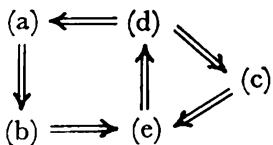
\includegraphics[keepaspectratio]{images/part001_f1dfd2f3.jpg}}

\begin{enumerate}
\def\labelenumi{(\alph{enumi})}
\item
  \(\Rightarrow\) (b): We know that a finitely generated projective module is finitely presented (Chapter I, § 2, no. 8, Lemma 8 (iii)); if P is a projective A-module, \(P_{m} = P \otimes_{A} A_{m}\) is a projective \(A_{m}\) -module (Algebra, Chapter II, § 5, no. 1, Corollary to Proposition 4); finally, as \(A_{m}\) is a local ring, every finitely presented projective \(A_{m}\) -module is free (§ 3, no. 2, Corollary to Proposition 5).
\item
  \(\Rightarrow\) (e): This follows from the Corollary to Proposition 2 of no. 1.
\item
  \(\Rightarrow\) (e): Let \(m\) be a maximal ideal of \(A\) ; write \(r_m = n\) and let \((x_i)_{1 \leqslant i \leqslant n}\) be a basis of \(P_m\) . We can assume that the \(x_i\) are canonical images of elements \(p_i \in P\) ( \(1 \leqslant i \leqslant n\) ) to within multiplication by an invertible element of \(A_m\) . Let \((e_i)_{1 \leqslant i \leqslant n}\) be the canonical basis of \(A^n\) and \(u: A^n \to P\) the homomorphism such that \(u(e_i) = p_i\) for \(1 \leqslant i \leqslant n\) . As \(P\) is finitely generated, it follows from Proposition 2 of no. 1 that there exists \(f \in A - m\) such that \(u_f\) is surjective. We conclude that \(u_{fg}\) is also surjective for all \(g \in A - m\) and by hypothesis there exists \(g \in A - m\) such that \(r_p = n\) for \(p \in X_g\) . Then, replacing \(f\) by \(fg\) , we may assume that \(r_p = n\) for all \(p \in X_f\) . Then \(u_p: A_p^n \to P_p\) is a surjective homomorphism and \(P_p\) and \(A_p\) are both free \(A_p\) -modules of the same rank; hence (§ 3, no. 2, Corollary to Proposition 6) \(u_p\) is bijective for all \(p \in X_f\) . Let \(p'\) be a prime ideal of \(A_f\) and let \(p\) be its inverse image in \(A\) under the canonical mapping; if \((A_f^n)_{p'}\) and \((P_f)_{p'}\) are identified with \(A_p^n\) and \(P_p\) under the canonical isomorphisms, \((u_f)_{p'}\) is identified with \(u_p\) and is consequently bijective. We conclude that \(u_f\) is bijective (§ 3, no. 3, Theorem 1), which establishes (e).
\item
  \(\Rightarrow\) (d): Let E be the set of \(f\in A\) such that \(\mathbf{P}_f\) is a finitely generated free \(\mathbf{A}_f\) -module. The hypothesis implies that E is contained in no maximal ideal of A, hence E generates the ideal A and there therefore exist a finite family \((f_{i})_{1 \leqslant i \leqslant n}\) of elements of E and \(a_{i} \in \mathbf{A}\) ( \(1 \leqslant i \leqslant n\) ) such that \(1 = \sum_{i=1}^{n} a_{i} f_{i}\) ; whence (d).
\item
  \(\Rightarrow\) (c): It follows from no. 1, Corollary to Proposition 3 that P is finitely generated. On the other hand, for every prime ideal p of A, there exists an index \(i\) such that \(\mathfrak{p} \in \mathrm{X}_{f_i}\) ; if \(\mathfrak{p}' = \mathfrak{p}_{f_i}\) , then \(\mathrm{P}_{\mathfrak{p}} = (\mathrm{P}_{f_i})_{\mathfrak{p}'}\) (§ 2, no. 5, Proposition
\end{enumerate}

\begin{enumerate}
\def\labelenumi{\arabic{enumi})}
\setcounter{enumi}{9}
\tightlist
\item
  and hence by hypothesis \(\mathbf{P}_{\mathfrak{p}}\) is free and of the same rank as \(\mathbf{P}_{f_i}\) , which proves (c).
\end{enumerate}

\begin{enumerate}
\def\labelenumi{(\alph{enumi})}
\setcounter{enumi}{3}
\tightlist
\item
  \(\Rightarrow\) (a): Consider the ring \(\mathbf{B} = \prod_{i\in I}\mathbf{A}_{f_i}\) and the B-module
\end{enumerate}

\[
\mathbf {M} = \prod_ {i \in I} \mathrm{P} _ {f _ {i}} = \mathrm{P} \otimes_ {\mathbf {A}} \mathrm{B}.
\]

For every index \(i\), there exists a free \(\mathbf{A}_{f_i}\)-module \(\mathbf{L}_i\) such that \(\mathbf{P}_{f_i}\) is a direct factor of \(\mathbf{L}_i\) and it may be assumed that all the \(\mathbf{L}_i\) have the same rank; then

\(L = \prod_{i \in I} L_i\) is a free B-module of which M is a direct factor, in other words M is a finitely generated projective B-module. As B is a faithfully flat A-module (no. 1, Proposition 3), we conclude that P is a finitely generated projective A-module (Chapter I, § 3, no. 6, Proposition 12).

COROLLARY 1. Suppose that the equivalent properties of the statement of Theorem 1 hold. Let \(m\) be an integer \(>0\) such that, for every family \((x_{i})_{1\leqslant i\leqslant m}\) of elements of \(\mathbf{P}\) , there exists a family \((a_{i})_{1\leqslant i\leqslant m}\) of elements of \(\mathbf{A}\) , which are not all divisors of zero and for which \(\sum_{i=1}^{m} a_i x_i = 0\) . Then, for all \(p \in \operatorname{Spec}(A)\) , \(r_p \leqslant m\) .

Let \(p\) be a prime ideal of \(A\); set \(r = r_p\), and let \((y_j)_{1 \leqslant j \leqslant r}\) be a basis of the free \(\mathbf{A}_{p}\)-module \(\mathbf{P}_{p}\). There exist elements \(x_j\) (\(1 \leqslant j \leqslant r\)) of \(\mathbf{P}\) and \(s \in A - p\) such that \(y_j = x_j / s\) for all \(j\). Then for every family \((a_j)_{1 \leqslant j \leqslant r}\) of elements of \(A\) such that \(\sum_{j=1}^{r} a_j x_j = 0\) , \(\sum_{j=1}^{r} (a_j / 1) y_j = 0\) in \(P_p\) , whence \(a_j / 1 = 0\) for \(1 \leqslant j \leqslant r\) . As \(A - p\) does not contain 0, this shows that the \(a_j\) are all divisors of zero in \(A\) ( \(\S 2\) , no. 1, Remark 3), hence of necessity \(r \leqslant m\) .

COROLLARY 2. Every finitely presented flat module is projective.\par

If P is a finitely presented flat A-module and m a maximal ideal of A, the \(A_{m}\) -module \(P_{m}\) is flat (§3, no. 4, Proposition 13) and finitely presented (§2, no. 4) and hence free (§3, no. 2, Corollary 2 to Proposition 5), Condition (b) of Theorem 1 therefore holds.

Remarks

\begin{enumerate}
\def\labelenumi{(\arabic{enumi})}
\item
  There exist finitely generated flat modules which are not projective (Exercise 7).
\item
  Corollary 2 to Theorem 1 extends to modules over non-commutative rings (Chapter I, § 2, Exercise 15).
\end{enumerate}
